\documentclass[11pt,letterpaper]{article}
\usepackage[T1]{fontenc}
\usepackage[utf8]{inputenc}
\usepackage{lmodern}
\usepackage[margin=1in,headheight=14pt]{geometry}
\usepackage{amsmath,amssymb,amsthm,mathtools}
\usepackage{booktabs,array,longtable}
\usepackage{graphicx,xcolor}
\usepackage{placeins}
\usepackage{enumitem}
\usepackage{microtype}
\usepackage{fancyhdr}
\usepackage{xurl}
\usepackage[colorlinks=true,linkcolor=blue!45!black,
 citecolor=blue!45!black,urlcolor=blue!45!black]{hyperref}
\usepackage[nameinlink,noabbrev]{cleveref}
\DeclareMathOperator{\Li}{Li}
\DeclareMathOperator{\GL}{GL}
\newtheorem{theorem}{Theorem}[section]
\newtheorem{proposition}[theorem]{Proposition}
\newtheorem{lemma}[theorem]{Lemma}
\newtheorem{corollary}[theorem]{Corollary}
\newtheorem{conjecture}[theorem]{Conjecture}
\theoremstyle{definition}
\newtheorem{definition}[theorem]{Definition}
\newtheorem{example}[theorem]{Example}
\theoremstyle{remark}
\newtheorem{remark}[theorem]{Remark}
\numberwithin{equation}{section}
\setlist{itemsep=3pt,topsep=5pt}
\setlength{\emergencystretch}{1.4em}
\setcounter{tocdepth}{2}
\pagestyle{fancy}
\fancyhf{}
\fancyhead[L]{\small ProveIt research continuation}
\fancyhead[R]{\small Golden seeds and analytic transitions}
\fancyfoot[C]{\thepage}
\hypersetup{
 pdftitle={Finite Golden Seeds and Uniform Analytic Transitions},
 pdfauthor={ProveIt research continuation prepared with OpenAI assistance},
 pdfsubject={Polylogarithms, signed Hausdorff measures, log-gamma moments, shuffle depth},
 pdfkeywords={polylogarithms, golden ratio, primitive divisors, signed moments,
 asymptotic analysis, shuffle algebra}}
\title{\textbf{Finite Golden Seeds and\\Uniform Analytic Transitions}\\[8pt]
 \large Multiplicative ladders, real-order signed kernels,\\
 reflected log-gamma moments, and a sharp depth obstruction}
\author{A research continuation for the ProveIt project\\
 \small Prepared with OpenAI assistance}
\date{10 October 2026}
\begin{document}
\maketitle
\begin{abstract}
We continue four lines of research in the current ProveIt polylogarithm
manuscript, distinguishing analytic identities, exact formal relations,
and numerical evidence. First, primitive-divisor theory reduces every
finite multiplicative seed for a positive real quadratic unit to indices
at most twelve or twenty-four, according to its norm. At the golden
reciprocal we determine the complete integral lattice: six generators
for all positive powers, four for even powers, and no rational seeds
after restricting the base to its fifth or any higher integer power.
This proves completeness of a historically known even-power alphabet,
without asserting sufficiency for higher-weight period identities.

Second, the coefficients \(H_{n-1}^{(b)}/n^a\), with real \(a,b>0\),
are moments of a finite signed measure exactly when \(a+b\ge1\).
Above the boundary the density has one simple sign change; on the
boundary it is strictly negative and a positive atom appears at one.
The measure gives a unique simple angular zero throughout the upper
half unit disk and a strictly increasing Cartesian abscissa.
We also determine the near-critical density crossing and the
concentration law of its positive mass.

Third, reflected log-gamma moments have a uniform transition at
\(n/(m+1)=\log m+O(1)\), with normalized limit
\(\exp(c e^{-s})\), where \(c=\zeta(2)/(2\gamma)-\gamma\).
We prove the first correction, an expansion to every fixed order,
and exact identities for near-diagonal residue polynomials.
Finally, a determinant-one certificate proves that the weight-six
binary shuffle quotient has exactly one direction beyond all
depth-two words and their six standard argument transforms.
Two explicit quotient identities follow.
The existing \(S_6\) special-value conjecture remains open.
The accompanying package supplies exact arithmetic replays,
independent analytic audits, numerical diagnostics, and proposed
editorial corrections.
\end{abstract}
\medskip
\noindent\textbf{Source snapshot.}
\href{https://github.com/VladimirReshetnikov/ProveIt/tree/28357e8ca63dd78327db91d9be239d75e4462879/Analysis/Polylogarithms/docs/manuscript}
{ProveIt manuscript, commit \texttt{28357e8ca63dd78327db91d9be239d75e4462879}}.
The source commit is dated 10 October 2026, 03:57:30 UTC.
\clearpage
\begingroup
\small
\tableofcontents
\endgroup
\clearpage

\section{Scope, results, and mathematical status}
\label{intro:sec}
The pinned source is already a substantial research manuscript
\cite{ProveIt}. It proves the \(S_4\) reduction, several all-weight
Gaussian and complementary-depth statements, algebraic low-weight
ladders, and a detailed fixed-reflected-exponent asymptotic theory.
We address four gaps: unbounded support
of multiplicative seeds, real orders and the boundary of signed-measure
representability, simultaneous growth of reflected exponents, and the
exact limitation of a natural depth-reduction vocabulary.

The source has several different notions of a relation. A relation
among algebraic units can be checked in a number field. A relation in
a formal shuffle or exterior-symbol quotient can be certified by
exact algebra. A numerical identity among special values requires an
analytic derivation or another valid equality proof. These notions
interact, but the implication from a formal relation to a numerical
period identity is not automatic. Every result below states the
space in which it is proved.

\subsection{A guide to the contributions}
\begin{center}
\small
\renewcommand{\arraystretch}{1.16}
\begin{tabular}{@{}>{\raggedright\arraybackslash}p{0.23\textwidth}>{\raggedright\arraybackslash}p{0.45\textwidth}>{\raggedright\arraybackslash}p{0.25\textwidth}@{}}
\toprule
Question & Result in this article & Nature of the conclusion\\
\midrule
Can larger golden exponents supply new multiplicative seeds?
& All finite relations have six explicit integral generators;
the even-power lattice has four.
& Unbounded arithmetic completeness,
Theorem~\ref{golden:thm:integral-lattice}.\\
Which real orders admit a finite signed moment measure?
& Exactly \(a+b\ge1\); the critical line has an endpoint atom.
& Analytic classification,
Theorem~\ref{real:thm:measure}.\\
Does the semicircle zero extend inside the disk?
& Exactly one simple angular zero at every radius;
its abscissa is strictly increasing.
& Analytic geometry,
Theorem~\ref{real:thm:arc}.\\
How does the critical atom form?
& Explicit crossing asymptotics and an exponential law on a
logarithmically rescaled coordinate.
& Uniform boundary analysis,
Section~\ref{real:sec:boundary}.\\
When does the fixed-\(m\) moment equivalent cease to be uniform?
& A nontrivial exponential profile occurs at
\(n/(m+1)-\log m=O(1)\).
& Uniform asymptotic theorem,
Theorem~\ref{moment:thm:transition}.\\
Can six standard argument changes remove all weight-six triples?
& Their depth-two span has codimension exactly one; two triple
combinations have explicit reductions.
& Formal quotient theorem,
Theorem~\ref{depthnew:thm:codimension}.\\
\bottomrule
\end{tabular}
\end{center}

The golden alphabet itself has historical precedent in
Bailey--Broadhurst \cite{BaileyBroadhurst1999}. The complete arithmetic
argument here uses Flatters' later primitive-divisor theorem
\cite{Flatters2009}. The log-gamma family is classical and is discussed
by Amdeberhan et al.\ \cite{Amdeberhan2011}; the new conclusion concerns
a growing second exponent in the regime explicitly left open by the
source. Li's recent positive-measure treatment of star polylogarithms
\cite{Li2026} provides nearby geometric context, while our measure is
signed and our indices are real.
Claims of extension in this article are relative to the pinned
manuscript and these identified sources. A complete literature search
for every consequence, or a claim of universal priority, is not intended.

\subsection{Conventions and proof architecture}
For \(|z|<1\) we use the strict convention
\[
 \Li_{s_1,\ldots,s_d}(z,1,\ldots,1)
 =\sum_{n_1>\cdots>n_d\ge1}
       \frac{z^{n_1}}{n_1^{s_1}\cdots n_d^{s_d}}.
\]
When exponents are real, the positive integer powers in the denominators
use the real logarithm. The notation \(\zeta(s,x)\) denotes the Hurwitz
zeta function and \(\gamma\) Euler's constant; standard gamma and zeta
identities use the conventions of the NIST DLMF \cite{DLMF}.
For boundary values of the real-order depth-two function, analytic
continuation on \(\mathbb C\setminus[1,\infty)\), equivalently radial
Abel limits away from \(1\), is used when the original series fails
to converge. Logarithms in the one-variable hyperlogarithm identities
are continued consistently from \(0<z<1\).

The arithmetic proof first rules out all sufficiently large indices,
then solves a finite integral lattice with explicit prime-ideal
witnesses. This order is essential: a finite search alone would not
prove completeness. The signed-kernel proof preserves the cancellation
at the origin of its defining integral. At the critical line the
usual Fubini argument is replaced by a differentiated Laplace identity,
which determines the missing atom. The moment proof similarly avoids
a tempting unjustified interchange: its uniform limit comes from a
weighted gamma-distribution integral, not a summation of the divergent
fixed-\(m\) pole expansion. The depth theorem specifies its formal
quotient before using exact ranks.

The analytic proofs have been independently reviewed within this
research workflow. Their review notes and finite arithmetic receipts
are included in the package. This is not formal verification in a
proof assistant or a substitute for external mathematical review.
Floating-point checks are diagnostics throughout; none is used to
promote a conjectural special-value identity to a theorem.

\section{Complete multiplicative seeds at the golden base}
\label{golden:sec:complete-seeds}

The complementary-power classification in the current manuscript
\cite{ProveIt} concerns relations of the form $r^a+r^b=1$.
Golden ladders also use products of many factors $1-r^n$.
We now give a completeness theorem for all such finite multiplicative
relations at the golden base, without imposing an exponent bound in
advance.  The result determines an integral relation lattice, explains
the eight arguments in the manuscript's higher golden formulas, and
classifies which integer powers of the base retain any such seeds.

The four exceptional indices $1,6,10,12$, when the base is the square
of the golden reciprocal, were already recorded by Bailey and
Broadhurst \cite[\S2, preceding (22)]{BaileyBroadhurst1999}.
We do not claim discovery of that list.  The contribution here is its
unbounded completeness proof, an explicit integral lattice for all
positive powers, and its consequences for power restrictions and
exterior symbols.  The arithmetic input is Flatters' later theorem
on primitive divisors \cite{Flatters2009}.

\subsection{An effective bound for every real quadratic unit}
\label{golden:subsec:quadratic-cutoff}

Let $K$ be a real quadratic field, let $\sigma$ denote its nontrivial
automorphism, and let $r\in\mathcal O_K^\times$ satisfy $0<r<1$.
Put $V_n(r)=1-r^n$ for $n\ge1$.
A prime ideal $\mathfrak p$ is \emph{primitive for $V_n(r)$} if it
divides $V_n(r)$ and none of $V_1(r),\ldots,V_{n-1}(r)$.
Because $r$ is a unit, this says exactly that its residue in the finite
field $\mathcal O_K/\mathfrak p$ has multiplicative order $n$.

We use the following part of Flatters' theorem: if $u$ is a positive
real quadratic unit of norm $+1$, then
$N_{K/\mathbb Q}(u^m-1)$ has a primitive rational prime divisor for
every $m>12$ \cite[Theorem~1.4]{Flatters2009}.
Here a rational prime is primitive if it divides this norm and no
earlier nonzero norm.  The following passage to prime ideals is needed
when the original unit has norm $-1$.

\begin{theorem}[Uniform quadratic cutoff]
\label{golden:thm:quadratic-cutoff}
If $N_{K/\mathbb Q}(r)=+1$, then $1-r^n$ has a primitive prime-ideal
divisor for every $n>12$.  If $N_{K/\mathbb Q}(r)=-1$, it has one
for every $n>24$.

Consequently, in any finite relation
\begin{equation}
 \prod_{n\ge1}(1-r^n)^{c_n}=r^b,
 \qquad c_n,b\in\mathbb Z,
 \label{golden:eq:general-seed}
\end{equation}
all coefficients above $12$ vanish in the norm $+1$ case, and all
coefficients above $24$ vanish in the norm $-1$ case.
The same support conclusion holds for rational exponents.
\end{theorem}

\begin{proof}
For norm $+1$, apply Flatters' theorem to $u=r^{-1}>1$.
At index $n>12$, choose a primitive rational divisor $p$ of
$N_{K/\mathbb Q}(u^n-1)$ and a prime ideal $\mathfrak p$ above $p$
dividing $u^n-1$.  The residue order of $u$ is exactly $n$: an order
$j<n$ would make $p$ divide the earlier norm
$N_{K/\mathbb Q}(u^j-1)$.  Inversion preserves order, so $r$ also
has order $n$ at this ideal.

For norm $-1$, put $q=r^2$ and apply the norm $+1$ theorem to
$u=r^{-2}$.  For each $m>12$, we obtain a primitive rational divisor
of $N_{K/\mathbb Q}(q^m-1)$, because
$u^j-1=-q^{-j}(q^j-1)$ differs by a unit.  At a suitable ideal
$\mathfrak p$ above this prime, the residue of $q$ has exact order
$m$.

The residue characteristic is odd.  Indeed, the residue field of an
ideal above $2$ in a quadratic field has size $2$ or $4$; the residue
of any unit therefore has order $1$ or $3$.  Thus $2$ divides some
norm $N_{K/\mathbb Q}(q^j-1)$ with $j\le3$, and cannot be
primitive at $m>12$.

Let $a$ be the residue of $r$ at $\mathfrak p$.  Since $a^2$ has
order $m$, the order of $a$ is either $m$ or $2m$, and it must be
$2m$ when $m$ is even.  The conjugation formula
\begin{equation}
 \sigma(r)=-r^{-1}
 \label{golden:eq:normminus-conjugation}
\end{equation}
identifies the residue of $r$ at the conjugate ideal, under the
induced field isomorphism, with $-a^{-1}$.  When $m$ is odd, these
two residues have orders $m$ and $2m$ in some order.  To check this
directly, if $a$ has odd order $m$, then $-a^{-1}$ has order $2m$.
If $a$ has order $2m$, then $a^m=-1$ in odd characteristic, so
$(-a^{-1})^m=1$; its square still has order $m$, forcing its order
to be $m$.
In this odd-$m$ case the ideals must be distinct: if they coincided,
the induced residue-field automorphism would preserve order.  Thus
no splitting assumption is needed.

For an even target $n>24$, take $m=n/2>12$.  If $m$ is even, the
chosen ideal gives residue order $n$.  If $m$ is odd, the chosen
ideal or its conjugate gives order $2m=n$.  For an odd target
$n>24$, take $m=n$ and choose the ideal giving order $m=n$.
This proves the prime-ideal statement in every case.

Finally, suppose \eqref{golden:eq:general-seed} has a nonzero
coefficient above the relevant cutoff, and choose its largest
supported index $N$.  At a primitive ideal for $V_N(r)$, all lower
factors and the unit $r$ have valuation zero.  Taking valuations gives
$c_N v_{\mathfrak p}(V_N(r))=0$, which contradicts both $c_N\ne0$
and $v_{\mathfrak p}(V_N(r))>0$.  Clearing denominators proves the
rational-exponent version.
\end{proof}

This theorem bounds multiplicative seeds.  It does not place an
unconditional bound on the weight of all polylogarithmic identities.
For a fixed quadratic base, it reduces seed determination to finitely
many exact ideal valuations and a unit calculation.

\subsection{The full integral lattice at the golden reciprocal}
\label{golden:subsec:integral-lattice}

Set
\[
 \rho=\frac{\sqrt5-1}{2},\qquad V_n=1-\rho^n,
 \qquad K=\mathbb Q(\sqrt5),\qquad\mathcal O_K=\mathbb Z[\rho].
\]
All $V_n$ are positive, so the following equations have no real
logarithm or sign ambiguity.

\begin{theorem}[Complete golden seed lattice]
\label{golden:thm:integral-lattice}
The group of finite integer relations
\begin{equation}
 \prod_{n\ge1}V_n^{c_n}=\rho^b,
 \qquad (c_n)\in\mathbb Z^{(\mathbb Z_{>0})},\quad b\in\mathbb Z,
 \label{golden:eq:rho-seed}
\end{equation}
is free of rank six.  An integral basis is
\begin{equation}
\begin{aligned}
 V_1&=\rho^2,&
 V_2&=\rho,\\
 V_6&=\rho^{-1}V_3^2,&
 V_{12}&=\rho^{-2}V_4V_3^3,\\
 V_{20}&=\rho^{-1}V_4^3V_{10},&
 V_{24}V_4&=\rho^{-2}V_3^4V_8^2.
\end{aligned}
\label{golden:eq:six-generators}
\end{equation}
Equivalently, $c$ occurs in \eqref{golden:eq:rho-seed} precisely when
its support is contained in
\begin{equation}
 S=\{1,2,3,4,6,8,10,12,20,24\}
 \label{golden:eq:full-support}
\end{equation}
and
\begin{equation}
\begin{aligned}
 c_3+2c_6+3c_{12}+4c_{24}&=0,\\
 c_4+c_{12}+3c_{20}-c_{24}&=0,\\
 c_8+2c_{24}&=0,\\
 c_{10}+c_{20}&=0.
\end{aligned}
\label{golden:eq:four-constraints}
\end{equation}
The uniquely determined unit exponent is
\begin{equation}
 b=2c_1+c_2-c_6-2c_{12}-c_{20}-2c_{24}.
 \label{golden:eq:unit-exponent}
\end{equation}
\end{theorem}

We first record the exact finite information needed in the proof.
Reducing powers using $\rho^2=1-\rho$ gives
\begin{center}
\small
\begin{tabular}{c|c@{\qquad}c|c}
$n$ & $V_n$ & $n$ & $V_n$\\ \hline
$1$ & $\rho^2$ & $2$ & $\rho$\\
$3$ & $2\rho^2$ & $4$ & $\sqrt5\rho^2$\\
$6$ & $4\rho^3$ & $8$ & $3\sqrt5\rho^4$\\
$10$ & $11\rho^5$ & $12$ & $8\sqrt5\rho^6$\\
$20$ & $55\sqrt5\rho^{10}$ & $24$ & $144\sqrt5\rho^{12}$
\end{tabular}
\end{center}
Substitution proves every equation in
\eqref{golden:eq:six-generators}.  In particular, the indices
\[
 E=\{1,2,6,12,20,24\}
\]
introduce no prime ideal absent from lower indices.

Every other index through $24$ has the following primitive witness.
A scalar $a$ denotes the ideal $(p,\rho-a)$ with residue field
$\mathbb F_p$.  The entry $\theta$ denotes the ideal $(p)$ with
residue field
$\mathbb F_p[\theta]/(\theta^2+\theta-1)$; the defining polynomial
is irreducible for the three primes $p=2,3,7$ used below.
All powers in the last column are computed in the indicated residue
field.

\begin{center}
\small
\begin{tabular}{r|r|r|l}
$n$ & $p$ & residue of $\rho$ & proper-power checks\\ \hline
$3$ & $2$ & $\theta$ & $\theta^1=\theta$\\
$4$ & $5$ & $2$ & $2^2=4$\\
$5$ & $11$ & $3$ & $3^1=3$\\
$7$ & $29$ & $23$ & $23^1=23$\\
$8$ & $3$ & $\theta$ & $\theta^4=2$\\
$9$ & $19$ & $4$ & $4^3=7$\\
$10$ & $11$ & $7$ & $7^5=10,\quad 7^2=5$\\
$11$ & $199$ & $61$ & $61^1=61$\\
$13$ & $521$ & $421$ & $421^1=421$\\
$14$ & $29$ & $5$ & $5^7=28,\quad5^2=25$\\
$15$ & $31$ & $18$ & $18^5=25,\quad18^3=4$\\
$16$ & $7$ & $\theta$ & $\theta^8=6$\\
$17$ & $3571$ & $1103$ & $1103^1=1103$\\
$18$ & $19$ & $14$ & $14^9=18,\quad14^6=7$\\
$19$ & $9349$ & $7563$ & $7563^1=7563$\\
$21$ & $211$ & $178$ & $178^7=196,\quad178^3=144$\\
$22$ & $199$ & $137$ & $137^{11}=198,\quad137^2=63$\\
$23$ & $139$ & $63$ & $63^1=63$
\end{tabular}
\end{center}

For each scalar row, direct arithmetic verifies
$a^2+a-1=0$ and $a^n=1$ modulo $p$; for each quadratic row it
verifies $\theta^n=1$.  The last column lists the values at $n/\ell$
for every prime $\ell\mid n$, and none equals $1$.
Thus the order is exactly $n$.  The listed rational primes are
verified by trial division, and irreducibility of the three quadratic
polynomials is checked by testing their residues.  The accompanying
script replays all of these finite checks in exact arithmetic.

\begin{proof}[Proof of Theorem~\ref{golden:thm:integral-lattice}]
Theorem~\ref{golden:thm:quadratic-cutoff} shows that every relation
\eqref{golden:eq:rho-seed} is supported on indices at most $24$.
Subtract integer multiples of the six rows in
\eqref{golden:eq:six-generators} to set the coefficients at
$1,2,6,12,20,24$ to zero.  Each row has coefficient $+1$ in its
own distinct pivot column and zero in every other pivot column, so
this elimination is integral and leaves all eliminated coefficients
zero.

If the residual relation is nonzero, let $N$ be its largest supported
index.  Then $N\notin E$ and the table supplies an ideal primitive
for $V_N$.  Every lower factor and $\rho$ has valuation zero there,
whereas $V_N$ has positive valuation.  Applying this valuation again
contradicts the nonzero coefficient at $N$.  Hence the six rows span
the entire relation group over $\mathbb Z$.

Their distinct pivot columns also prove independence.  Reading their
other columns gives \eqref{golden:eq:four-constraints}, and reading
their unit exponents gives \eqref{golden:eq:unit-exponent}.  The unit
exponent is unique because $\rho$ is not a root of unity.
\end{proof}

\begin{remark}[Why the ideal witnesses matter]
The norms of $V_5$ and $V_{10}$ are $11$ and $-121$.
One ideal above $11$ has residue $\rho=3$ of order $5$; its conjugate
has residue $\rho=7$ of order $10$.  Thus $V_{10}$ has a primitive
prime-ideal divisor even though its norm has no primitive rational
prime divisor.  A proof using only new rational prime factors of the
norms would miss this constraint.
\end{remark}

\subsection{Four even-power seeds and an integral parity condition}
\label{golden:subsec:even-seeds}

Put $q=\rho^2$ and $U_j=1-q^j=V_{2j}$.

\begin{corollary}[The complete even-power lattice]
\label{golden:cor:even-seeds}
All finite integral relations
$\prod_{j\ge1}U_j^{c_j}=\rho^b$ are generated freely by
\begin{equation}
\begin{aligned}
 U_1&=\rho,\\
 U_6^2&=\rho^{-1}U_2^2U_3^3,\\
 U_{10}&=\rho^{-1}U_2^3U_5,\\
 U_{12}U_2&=U_3^2U_4^2.
\end{aligned}
\label{golden:eq:four-even-generators}
\end{equation}
Their support is contained in
\begin{equation}
 \{1,2,3,4,5,6,10,12\}
 \quad\text{in the $q$ index}.
 \label{golden:eq:even-support}
\end{equation}
If the four rows are used with multiplicities $(A,B,C,D)$,
the resulting exponent of $\rho$ is $A-B-C$.
The result is an integer power of $q$ precisely when $A-B-C$ is even.
\end{corollary}

\begin{proof}
Write the multiplicities of the rows in
\eqref{golden:eq:six-generators} as
$a_1,a_2,a_6,a_{12},a_{20},a_{24}$.
Their odd-index coefficients vanish exactly when
\[
 a_1=0,\qquad 2a_6+3a_{12}+4a_{24}=0.
\]
Thus $a_{12}$ is even and
$a_6=-3(a_{12}/2)-2a_{24}$.
The four free integer parameters
$a_2,a_{12}/2,a_{20},a_{24}$ give exactly
\eqref{golden:eq:four-even-generators}.  The unit exponent follows
from the four displayed identities, proving the parity assertion.
\end{proof}

The support \eqref{golden:eq:even-support} is precisely the
eight-argument set
\begin{equation}
 \mathcal A=\{\rho^2,\rho^4,\rho^6,\rho^8,
                 \rho^{10},\rho^{12},\rho^{20},\rho^{24}\}
 \label{golden:eq:manuscript-alphabet}
\end{equation}
used by the manuscript's conjectured higher-weight golden ladders.
The theorem now establishes that no arbitrarily large even exponent
can introduce another multiplicative seed.  At the level of rational
logarithmic relations, the integral parity condition disappears because
$\mathbb Q\log q=\mathbb Q\log\rho$.

\subsection{Which powers of the base retain any seeds?}
\label{golden:subsec:power-restriction}

For a positive integer $h$, define the rational relation space
\begin{equation}
 \mathcal R_h=
 \left\{(c_n)\in\mathbb Q^{(\mathbb Z_{>0})}:
  \sum_{n\ge1}c_n\log(1-\rho^{hn})
      \in\mathbb Q\log\rho\right\}.
 \label{golden:eq:restricted-space}
\end{equation}
One may replace the line $\mathbb Q\log\rho$ by
$\mathbb Q\log(\rho^h)$ without changing this space.

\begin{theorem}[Sharp power-restriction ranks]
\label{golden:thm:power-ranks}
For every positive integer $h$,
\begin{equation}
 \dim_{\mathbb Q}\mathcal R_h=
 \begin{cases}
 6,&h=1,\\
 4,&h=2,\\
 1,&h=3,4,\\
 0,&h\ge5.
 \end{cases}
 \label{golden:eq:power-ranks}
\end{equation}
For $h=3$, the unique rational direction is
$V_6/V_3^2=\rho^{-1}$.
For $h=4$, it is
\begin{equation}
 \frac{V_{12}^4V_8^6}{V_4^7V_{24}^3}=\rho^{-2}.
 \label{golden:eq:power-four-direction}
\end{equation}
The primitive integral relations whose right sides are integer powers
of their own base $r=\rho^h$ are
\begin{align}
 h=3:\quad &(1-r^2)^3=r^{-1}(1-r)^6,
 \label{golden:eq:power-three-integral}\\
 h=4:\quad &(1-r^3)^8(1-r^2)^{12}
       =r^{-1}(1-r)^{14}(1-r^6)^6.
 \label{golden:eq:power-four-integral}
\end{align}
\end{theorem}

\begin{proof}
Clear denominators in \eqref{golden:eq:restricted-space} and
exponentiate.  The resulting relation has the form
\eqref{golden:eq:rho-seed} and is supported only on multiples of $h$.
Theorem~\ref{golden:thm:integral-lattice} supplies the complete
support and constraints.

The cases $h=1,2$ follow immediately from that theorem and
Corollary~\ref{golden:cor:even-seeds}.
For $h=3$, the permitted support is $\{3,6,12,24\}$.
The equation at index $8$ in \eqref{golden:eq:four-constraints}
forces $c_{24}=0$; the equation at index $4$ then forces
$c_{12}=0$.  The remaining freedom is $c_3=-2c_6$.

For $h=4$, the permitted support is $\{4,8,12,20,24\}$.
The equation at index $10$ forces $c_{20}=0$; that at index $3$
gives $3c_{12}+4c_{24}=0$.
Thus the integer solutions are
\[
 c_{12}=4t,\qquad c_{24}=-3t,\qquad
 c_4=-7t,\qquad c_8=6t,
\]
which give \eqref{golden:eq:power-four-direction}.
Their unit exponent is $-2t$, so it is an integer power of
$\rho^4$ precisely when $t$ is even.  For $h=3$, the unit
exponent is $-c_6$, so an integer power of $\rho^3$ requires
$3\mid c_6$.  These conditions give the two primitive integral
relations displayed in the theorem.

For $h\ge5$, support is empty unless $h$ divides a member of
$S$ in \eqref{golden:eq:full-support}.  The possibilities are
$h\in\{5,6,8,10,12,20,24\}$.  It suffices to exclude $5,6,8$,
as their multiples impose further restrictions.
For $h=5$, only indices $10,20$ are permitted; the index-$4$
equation forces $c_{20}=0$, and the index-$10$ equation then
forces $c_{10}=0$.
For $h=6$, only $6,12,24$ are permitted; the equations at indices
$8,4,3$ eliminate them in that order.
For $h=8$, only $8,24$ are permitted; the equation at index $4$
eliminates $24$, then that at index $8$ eliminates $8$.
This proves all cases of \eqref{golden:eq:power-ranks}.
\end{proof}

The number field remains $\mathbb Q(\sqrt5)$ under these power
substitutions, but the permitted positive-power seed space can shrink
from dimension six to zero.  Thus the field alone does not determine
the seed count for a specified base and argument family.

\subsection{All-weight kernels of the exterior-symbol map}
\label{golden:subsec:exterior-symbol}

Put
\[
 W=K^\times\otimes_{\mathbb Z}\mathbb Q,
 \qquad\langle x\rangle=x\otimes1\in W,
 \qquad v=\langle\rho\rangle,
\]
and use additive notation for $W$.
For $w\ge2$, define the rationalized classical exterior-symbol map
\begin{equation}
 \beta_w([x])=
 \langle x\rangle^{\otimes(w-2)}\otimes
 \bigl(\langle x\rangle\wedge\langle1-x\rangle\bigr)
 \quad (x\ne0,1),
 \label{golden:eq:beta-definition}
\end{equation}
with target $W^{\otimes(w-2)}\otimes\bigwedge^2W$.
Here $[x]$ denotes a generator in a free rational vector space.
We make no identification of its quotient with numerical periods.

\begin{theorem}[Complete positive-power exterior-symbol kernels]
\label{golden:thm:symbol-kernel}
On the free span of $[\rho^n]$, $n\ge1$, the kernel of $\beta_w$
has dimension six at every weight $w\ge2$.
An explicit basis consists of
\begin{equation}
 \sum_n\frac{c_n}{n^{w-1}}[\rho^n],
 \label{golden:eq:weighted-seed}
\end{equation}
where $c$ runs through the six coefficient vectors in
\eqref{golden:eq:six-generators}.
Every kernel element is supported on
\eqref{golden:eq:full-support}.
On even powers the kernel has dimension four and is supported on
\eqref{golden:eq:manuscript-alphabet}.
On the span of $[\rho^{hn}]$, its dimensions are
\eqref{golden:eq:power-ranks}.
\end{theorem}

\begin{proof}
The vector $v$ is nonzero because $\rho$ is not torsion.
Multilinearity gives, for every finitely supported rational vector $a$,
\begin{equation}
 \beta_w\!\left(\sum_n a_n[\rho^n]\right)
 =v^{\otimes(w-2)}\otimes
 \left(v\wedge\sum_n a_n n^{w-1}\langle V_n\rangle\right).
 \label{golden:eq:beta-factorization}
\end{equation}
Tensoring over a field with a fixed nonzero pure tensor is injective,
and $v\wedge z=0$ if and only if $z\in\mathbb Qv$.
Consequently \eqref{golden:eq:beta-factorization} vanishes exactly
when
\begin{equation}
 \sum_n a_n n^{w-1}\langle V_n\rangle\in\mathbb Qv.
 \label{golden:eq:weighted-line-test}
\end{equation}

After clearing denominators, this says that a positive real algebraic
number $\prod_nV_n^{c_n}\rho^{-b}$ is torsion.  A positive real
root of unity is $1$, so the condition is equivalent to the actual
multiplicative relation \eqref{golden:eq:rho-seed}, with the
coefficients proportional to $a_n n^{w-1}$.
The diagonal operation $a_n\mapsto n^{w-1}a_n$ is invertible and
preserves support.  Theorems~\ref{golden:thm:integral-lattice}
and \ref{golden:thm:power-ranks} therefore give the basis, support,
and every stated dimension.
\end{proof}

\paragraph{Scope of the obstruction.}
This theorem computes the kernel of the explicitly specified algebraic
map.  A nonzero exterior symbol rules out a certificate requiring
vanishing in this map.  Vanishing in the number-field symbol alone does
not supply a rational-function deformation, lower-weight compatibility,
or the regulator information needed to prove a higher polylogarithm
identity.  In particular, dimension four does not assert that four
numerical ladders exist at every weight, and it does not prove that
none exists above weight nine.  Numerical period independence remains
a separate arithmetic question.

The constructive consequence is that searches beginning with this
symbol can use \eqref{golden:eq:manuscript-alphabet} as a complete
even-power alphabet and work in four weighted seed coordinates.
Increasing the positive even exponents beyond $24$ cannot enlarge that
particular kernel.

\subsection{Exact replay and next proof problems}
\label{golden:subsec:replay}

The file \texttt{code/golden\_seed\_certificate.py} uses only
Python's standard library.  It verifies the six generator identities
in $\mathbb Q[X]/(X^2+X-1)$, the two primitive own-base relations
at $h=3,4$, all eighteen primitive prime-ideal witnesses, and the
rational restriction ranks for $1\le h\le25$.
The output is preserved in
\texttt{data/golden\_seed\_certificate.json}.
Every calculation in this replay uses exact integer or rational
arithmetic.  The infinite bounds rest on Flatters' theorem and the
prime-ideal argument above; the proof for all $h\ge5$ rests on the
explicit support constraints.

Several further questions are now more sharply delimited.
First, the unresolved golden formulas at weights five through nine
can be approached in the complete eight-argument symbol alphabet;
the missing step is an exact functional-equation or regulator
certificate.  Second, the same uniform $12/24$ cutoff permits complete
seed computations for other real quadratic units, retaining the unit
index congruence when the base is not fundamental.
Third, an effective prime-ideal cutoff for the cubic plastic and
supergolden fields would give an analogous completeness theorem there.
Finally, formalization can begin with the finite arithmetic interface:
quadratic algebra, exact residue orders, integral elimination, and
the tensor/exterior linear-algebra argument.  The cited
primitive-divisor theorem is an explicit separate dependency.

\section{Real-weight signed kernels and a sharp measure threshold}
\label{real:sec:kernels}

The signed-kernel chapter of the pinned manuscript proves that the strict
depth-two coefficients $H_{n-1}^{(b)}/n^a$, with integer $a\geq1$ and real
$b>0$, have an integrable density with one sign change. That structure
gives a unique zero of the imaginary part on the upper semicircle.
The affine signed-moment continuation already permits real $a\geq1$
for measure existence and total-variation estimates, but does not extend
the one-crossing theorem to that range or treat $0<a<1$~\cite{ProveIt}.
We now classify the complete domain of finite signed measures for these
coefficients. Its boundary has a positive endpoint atom, and requires a
different cancellation argument from the interior.

Hausdorff--Stieltjes methods for polylogarithmic geometry have substantial
existing context. In particular, Li's recent work treats positive
Hausdorff measures and likelihood-ratio ordering for integer-index
multiple \emph{star} polylogarithms~\cite{Li2026}. Here the strict
depth-two sequence has total moment mass zero, so its representing
measure is signed. The results below concern real exponents, the sharp
boundary of finite-measure representability, and the associated zero
arc. The claim of extension is relative to the pinned manuscript; no
complete priority claim is intended.

For $a,b>0$ define
\begin{equation}\label{real:eq:def}
 m_n(a,b)=\frac{H_{n-1}^{(b)}}{n^a},\qquad
 H_{n-1}^{(b)}=\sum_{j=1}^{n-1}j^{-b},\qquad
 F_{a,b}(z)=\sum_{n\geq1}m_n(a,b)z^n\quad(|z|<1).
\end{equation}
The empty harmonic sum is zero. At integer exponents $F_{a,b}$ is the
strict depth-two polylogarithm used in the source manuscript.

\subsection{A real-order kernel with cancellation retained}

For $T>0$ put
\begin{equation}\label{real:eq:kernel}
\begin{split}
 k_{a,b}(T)={}&-\frac{T^{a+b-1}}{\Gamma(a+b)}\\
 &+\frac1{\Gamma(a)\Gamma(b)}
  \int_0^\infty\frac{v^{b-1}}{e^v-1}
    \bigl[T^{a-1}-(T-v)_+^{a-1}\bigr]\,dv,
\end{split}
\end{equation}
and $\kappa_{a,b}(u)=k_{a,b}(-\log u)$ for $0<u<1$.
Here $(T-v)_+^{a-1}$ means $(T-v)^{a-1}$ when $v<T$, and zero when
$v>T$; its value at $v=T$ is irrelevant. In particular, if $0<a<1$,
the left-hand singularity at $v=T$ is retained. The integral converges
absolutely for each fixed $T$: its bracket is $O_T(v)$ at zero, the
singularity at $v=T$ has integrable exponent $a-1>-1$, and the tail
decays exponentially. For $b\leq1$ the two terms inside the bracket
must remain combined near $v=0$.

\begin{theorem}[Sharp finite signed-measure classification]
\label{real:thm:measure}
Let $a,b>0$. There is a finite signed Borel measure $\mu_{a,b}$ on
$[0,1]$ satisfying
\begin{equation}\label{real:eq:moments}
 \int_{[0,1]}u^{n-1}\,d\mu_{a,b}(u)=m_n(a,b),\qquad n\geq1,
\end{equation}
if and only if $a+b\geq1$. Whenever it exists, it is unique and has
total mass zero. More precisely:
\begin{enumerate}
\item If $a+b>1$, the measure is
$d\mu_{a,b}(u)=\kappa_{a,b}(u)\,du$, with $\kappa_{a,b}\in L^1(0,1)$.
There is a unique $r_{a,b}\in(0,1)$ such that
\begin{equation}\label{real:eq:signs}
 \kappa_{a,b}(u)<0\quad(0<u<r_{a,b}),\qquad
 \kappa_{a,b}(u)>0\quad(r_{a,b}<u<1).
\end{equation}
The zero is simple in the coordinate $T=-\log u$.
\item If $a+b=1$, then $0<a,b<1$ and
\begin{equation}\label{real:eq:atom}
 d\mu_{a,b}(u)=\frac1a\,d\delta_1(u)+\kappa_{a,b}(u)\,du.
\end{equation}
The same formula \eqref{real:eq:kernel} defines an integrable density,
and
\begin{equation}\label{real:eq:critical-density}
 \kappa_{a,b}(u)<-1\quad(0<u<1),\qquad
 \int_0^1\kappa_{a,b}(u)\,du=-\frac1a.
\end{equation}
Thus all positive mass is the endpoint atom $1/a$ at $u=1$.
\end{enumerate}
\end{theorem}

\begin{proof}
We prove convergence, signs, and the boundary atom separately.

\paragraph{Integrability and moments when $a+b>1$.}
For $n>0$, direct integration gives
\begin{equation}\label{real:eq:translate-laplace}
\begin{split}
 &\int_0^\infty e^{-nT}
  \bigl[T^{a-1}-(T-v)_+^{a-1}\bigr]\,dT\\
 &\hspace{25mm}=\Gamma(a)n^{-a}(1-e^{-nv}).
\end{split}
\end{equation}
If $a\geq1$, the bracket is nonnegative. Tonelli's theorem applies,
and at $n=1$ the positive integral contribution in
\eqref{real:eq:kernel} is exactly one. The explicit negative term has
absolute integral one against $e^{-T}\,dT$ as well.

If $0<a<1$, write
\[
 B_n(v)=\int_0^\infty e^{-nT}
  \left|T^{a-1}-(T-v)_+^{a-1}\right|\,dT.
\]
For $0<v\leq1$, split the $T$-integral at $2v$. The part before
$2v$ is $O(v^a)$. On $T\geq2v$, the mean value theorem bounds the
difference by $C_a vT^{a-2}$, whose integral is also $O(v^a)$.
Thus $B_n(v)=O(v^a)$ near zero. For $v\geq1$, separate gamma
integrals give $B_n(v)\leq C_n$. Since
$v^{b-1}/(e^v-1)=O(v^{b-2})$ at zero, the double absolute integral
converges if $a+b>1$. This proves integrability and justifies Fubini
in \eqref{real:eq:translate-laplace}. For integers $n\geq1$,
\begin{align}
 \int_0^\infty e^{-nT}k_{a,b}(T)\,dT
 &=-n^{-a-b}+\frac{n^{-a}}{\Gamma(b)}
  \int_0^\infty\frac{v^{b-1}(1-e^{-nv})}{e^v-1}\,dv\notag\\
 &=-n^{-a-b}+n^{-a}\sum_{j=1}^n j^{-b}
 =m_n(a,b).\label{real:eq:moment-evaluation}
\end{align}
The finite geometric identity
$(1-e^{-nv})/(e^v-1)=\sum_{j=1}^n e^{-jv}$ proves the second line.
The change of variable $u=e^{-T}$ gives
\eqref{real:eq:moments}; at $n=1$ it also gives zero total mass.

\paragraph{The crossing problem as a fixed positive level.}
Define
\begin{equation}\label{real:eq:scaled-integral}
 g(s)=s^{b-1}\bigl[1-(1-s)_+^{a-1}\bigr],\qquad
 I(T)=\int_0^\infty\frac{g(s)}{e^{Ts}-1}\,ds.
\end{equation}
Substitution $v=Ts$ gives
\begin{equation}\label{real:eq:level}
 \frac{k_{a,b}(T)}{T^{a+b-1}}
 =-\frac1{\Gamma(a+b)}+\frac{I(T)}{\Gamma(a)\Gamma(b)}.
\end{equation}
If $a\geq1$, then $g$ is nonnegative and positive on a set of
positive measure, so $I'(T)<0$.

If $0<a<1$, then $g<0$ on $(0,1)$ and $g>0$ on $(1,\infty)$.
For $T_2>T_1>0$ the ratio
\[
 R(s)=\frac{e^{T_1s}-1}{e^{T_2s}-1}
\]
is strictly decreasing in $s$ and satisfies $0<R(s)<1$.
Indeed, logarithmic differentiation reduces this assertion to the
strict increase of $t/(1-e^{-t})$ for $t>0$. If $I(T_1)=C>0$,
then
\[
 I(T_2)-R(1)I(T_1)
 =\int_0^\infty\frac{g(s)}{e^{T_1s}-1}
       \bigl(R(s)-R(1)\bigr)\,ds<0.
\]
Both parts of the integrand are strictly negative. Consequently
$I(T_2)<C$. When $T_2<T_1$, the ratio is instead strictly increasing
and exceeds one, yielding $I(T_2)>C$. Therefore $I$ crosses any
fixed positive level at most once.

At such a crossing the derivative is strictly negative. In fact,
\[
 q_T(s)=-\frac{s}{1-e^{-Ts}}
\]
is strictly decreasing and negative; subtracting $q_T(1)I(T)$ from
the differentiated integral gives
$I'(T)<q_T(1)I(T)<0$. All differentiations follow from domination on
compact positive $T$-intervals. Thus a crossing of the positive level
$\Gamma(a)\Gamma(b)/\Gamma(a+b)$ in \eqref{real:eq:level}, if it
exists, is unique and simple.

\paragraph{Endpoint signs.}
Dominated convergence in \eqref{real:eq:scaled-integral} shows that
$I(T)\to0$ as $T\to\infty$. Hence $k_{a,b}$ is negative for large
$T$. At the other endpoint one has
\begin{equation}\label{real:eq:endpoints}
 k_{a,b}(T)\sim
 \begin{cases}
 \displaystyle\frac{\zeta(b)}{\Gamma(a)}T^{a-1},&b>1,\\[5pt]
 \displaystyle\frac{T^{a-1}}{\Gamma(a)}\log(1/T),&b=1,\\[5pt]
 \displaystyle\frac{T^{a+b-2}}{(1-b)\Gamma(a+b-1)},
       &0<b<1, a+b>1.
 \end{cases}
\end{equation}
For the first two cases, divide \eqref{real:eq:kernel} by $T^{a-1}$
and split its integral at $v=T$. The part on $(0,T)$ is
$O(T^{b-1})$ after $v=Ts$: cancellation at $s=0$ and the exponent
$a-1>-1$ at $s=1$ give a finite constant. The remaining part is
$\int_T^\infty v^{b-1}/(e^v-1)\,dv$, which tends to
$\Gamma(b)\zeta(b)$ for $b>1$ and equals
$\log(1/T)+O(1)$ for $b=1$.

For $0<b<1$, the absolutely convergent beta identity
\begin{equation}\label{real:eq:beta}
 \int_0^\infty\frac{g(s)}s\,ds
 =\frac{a+b-1}{1-b}B(b,a)
\end{equation}
holds for every $a>0$. To prove it without analytic continuation,
first replace $a$ by $a+1$ and integrate by parts; this gives
$aB(b,a)/(1-b)$. On $(0,1)$ use
\[
 1-(1-s)^{a-1}=\bigl[1-(1-s)^a\bigr]-s(1-s)^{a-1}
\]
and subtract $B(b,a)$. These operations involve only convergent
integrals. Since $T/(e^{Ts}-1)\leq1/s$, dominated convergence gives
\[
 TI(T)\longrightarrow\frac{a+b-1}{1-b}B(b,a).
\]
For $a+b>1$, inserting this limit in \eqref{real:eq:level} proves
the third case of \eqref{real:eq:endpoints}. Thus $k_{a,b}$ is
positive near zero. Its unique simple crossing follows, and
$u=e^{-T}$ reverses the order of the signs as in
\eqref{real:eq:signs}.

\paragraph{The critical density.}
Suppose $a+b=1$. In this case $0<a,b<1$, and
\eqref{real:eq:beta} says that the integrable function
$c(s)=g(s)/s$ has zero integral. It is negative on $(0,1)$ and
positive on $(1,\infty)$. The function
\[
 q_T(s)=\frac{s}{e^{Ts}-1}
\]
is strictly decreasing. Subtracting $q_T(1)\int c=0$ therefore gives
$I(T)=\int c(s)q_T(s)\,ds<0$. Equation
\eqref{real:eq:level}, with $a+b=1$, proves $k_{a,b}(T)<-1$.

The critical integrability assertion needs cancellation. Use
$\int c=0$ and the elementary bound
\[
 0\leq\frac1T-\frac{s}{e^{Ts}-1}\leq\min(s,1/T).
\]
On $(0,1)$ the integral of $s|c(s)|$ is finite, while on
$[1,\infty)$ one has $c(s)=s^{b-2}$. Splitting the latter integral
at $1/T$ proves $|I(T)|=O(1+T^{-b})$ as $T\downarrow0$.
Since $b<1$, this is integrable in $T$. For $T\geq1$ the integral
has a fixed absolutely integrable majorant. Hence
$e^{-T}k_{a,b}(T)$ is integrable.

One cannot apply \eqref{real:eq:moment-evaluation} at this boundary:
its unweighted double absolute integral can fail to converge.
Instead introduce an additional factor $T$. Splitting at $2v$ as
before yields
\begin{equation}\label{real:eq:extra-T}
 \int_0^\infty T e^{-nT}
 \left|T^{a-1}-(T-v)_+^{a-1}\right|\,dT=O(v)
 \quad(v\downarrow0).
\end{equation}
The first part is $O(v^{a+1})$. The remaining part is bounded by
$C_av\int_{2v}^\infty T^{a-1}e^{-nT}\,dT=O(v)$.
The resulting double absolute integral converges for every $b>0$.

Define, now for any real $x>0$,
\begin{equation}\label{real:eq:interpolated-moment}
 m(x)=-x^{-a-b}+\frac{x^{-a}}{\Gamma(b)}
  \int_0^\infty\frac{v^{b-1}(1-e^{-xv})}{e^v-1}\,dv.
\end{equation}
For integer $x=n$, this is $m_n(a,b)$. Differentiating
\eqref{real:eq:translate-laplace}, with
\eqref{real:eq:extra-T} supplying Fubini's hypothesis, gives
\[
 \frac{d}{dx}\int_0^\infty e^{-xT}k_{a,b}(T)\,dT=m'(x).
\]
The difference between these functions is constant. The Laplace
integral tends to zero as $x\to\infty$, whereas elementary
sum--integral comparison gives
\[
 m_n(a,1-a)=n^{-a}H_{n-1}^{(1-a)}\longrightarrow\frac1a.
\]
Taking this limit along the integers determines the constant:
\begin{equation}\label{real:eq:critical-laplace}
 \int_0^\infty e^{-xT}k_{a,1-a}(T)\,dT=m(x)-\frac1a.
\end{equation}
This proves the endpoint atom in \eqref{real:eq:atom}. At $x=1$
it also gives the density mass in \eqref{real:eq:critical-density}.

\paragraph{Necessity and uniqueness.}
If $a+b<1$, then $b<1$ and
\[
 m_n(a,b)\sim\frac{n^{1-a-b}}{1-b}\longrightarrow+\infty.
\]
Moments of a finite signed measure on $[0,1]$ are bounded by its
total variation, a contradiction. Finally, polynomials are dense in
$C[0,1]$, so equality of all polynomial moments implies equality of
finite signed measures. This proves uniqueness and finishes the
classification.
\end{proof}

\begin{corollary}[A completely monotone critical deficit]
\label{real:cor:deficit}
For $0<a<1$ define
\begin{equation}\label{real:eq:deficit}
 d_a(x)=\frac1a-x^{-a}
       \bigl[\zeta(1-a)-\zeta(1-a,x)\bigr],\qquad x>0.
\end{equation}
Then $d_a(x)-1/x$ is strictly completely monotone. In particular, for
every integer $j\geq0$ and $x>0$,
\begin{equation}\label{real:eq:deficit-bound}
 (-1)^j d_a^{(j)}(x)>\frac{j!}{x^{j+1}}.
\end{equation}
The sequence $1/a-n^{-a}H_{n-1}^{(1-a)}$, $n\geq1$, is a positive
Hausdorff moment sequence, represented by the density
$-\kappa_{a,1-a}(u)>1$.
\end{corollary}
\begin{proof}
For $b=1-a$, the convergent difference integral
\[
 \zeta(b)-\zeta(b,x)
 =\frac1{\Gamma(b)}\int_0^\infty
  \frac{v^{b-1}(e^{-v}-e^{-xv})}{1-e^{-v}}\,dv
\]
identifies \eqref{real:eq:interpolated-moment} with
$x^{-a}[\zeta(b)-\zeta(b,x)]$.
Consequently \eqref{real:eq:critical-laplace} gives
\[
 d_a(x)=\int_0^\infty e^{-xT}\bigl[-k_{a,1-a}(T)\bigr]\,dT.
\]
The density is strictly greater than one. Differentiation is justified
by the endpoint bounds in the proof of Theorem~\ref{real:thm:measure}.
After $j$ derivatives the integral is strictly greater than
$\int_0^\infty T^j e^{-xT}\,dT=j!/x^{j+1}$.
Subtracting $1/x$ leaves the positive density $-k-1$, proving the
complete-monotonicity assertion. Integer $x$ gives the moment statement.
\end{proof}

\subsection{The entire zero arc in the upper half unit disk}

The finite-measure threshold also supports a complete geometric
statement. At the critical line, boundary values must be understood
analytically: the coefficients in \eqref{real:eq:def} tend to $1/a$,
so the unit-circle series does not converge in the ordinary sense.

\begin{theorem}[Unique simple angular zero at every radius]
\label{real:thm:arc}
Let $a,b>0$ with $a+b\geq1$. The function $F_{a,b}$ continues
holomorphically to $\mathbb C\setminus[1,\infty)$ by
\begin{equation}\label{real:eq:continuation}
 F_{a,b}(z)=\int_{[0,1]}\frac{z}{1-zu}\,d\mu_{a,b}(u).
\end{equation}
For each $0<R\leq1$, exactly one
$\theta_{a,b}(R)\in(0,\pi)$ satisfies
$\Im F_{a,b}(Re^{i\theta_{a,b}(R)})=0$. It is simple, its angular
derivative is negative, and
\begin{equation}\label{real:eq:arc-enclosure}
 \arccos R<\theta_{a,b}(R)<\frac\pi2.
\end{equation}
The imaginary part is positive before this zero and negative after
it as $\theta$ increases from $0$ to $\pi$.

Set $s=R^2$ and $x_{a,b}(s)=R\cos\theta_{a,b}(R)$. Then
$x_{a,b}$ is real analytic on $(0,1]$, extends real analytically
through $s=0$, and
\begin{equation}\label{real:eq:x-motion}
 0<x_{a,b}(s)<s,\qquad x_{a,b}'(s)>0\quad(0<s\leq1).
\end{equation}
\end{theorem}

\begin{proof}
Expanding the kernel of \eqref{real:eq:continuation} for $|z|<1$
and applying Theorem~\ref{real:thm:measure} proves the identity
there. On compact subsets of the slit plane its denominator is
bounded away from zero uniformly for $u\in[0,1]$, so the finite
measure proves holomorphy and continuation.

We use an elementary sign test. If a zero-mass signed measure has
its negative and positive parts separated, integration against a
strictly increasing function is strictly positive, and integration
against a strictly decreasing function is strictly negative.
Subtract the value of the test function at the separating point to
prove this. For $a+b>1$ use the crossing $r_{a,b}$ from
\eqref{real:eq:signs}. For $a+b=1$ use the separating point $1$:
the negative density lies in $(0,1)$ and the positive mass is at $1$.
Strictness still follows on the interval occupied by the density.

Write $c=\cos\theta$ and
\[
 K_c(u)=\frac1{1-2Rcu+R^2u^2},\qquad
 J_R(c)=\int_{[0,1]}K_c(u)\,d\mu_{a,b}(u).
\]
Then
\begin{equation}\label{real:eq:angular-J}
 \Im F_{a,b}(Re^{i\theta})=R\sin\theta\,J_R(\cos\theta).
\end{equation}
The kernel $K_0$ is strictly decreasing in $u$, so $J_R(0)<0$.
For $R<1$, an absolutely convergent geometric expansion gives
\begin{equation}\label{real:eq:positive-endpoint}
 J_R(1)=\sum_{k\geq0}(k+1)R^k m_{k+1}(a,b)
       \geq2R m_2(a,b)>0.
\end{equation}

For $R=1$ and $a+b>1$, split the measure at its sign crossing.
The negative part stays away from $u=1$, so its contribution has a
finite limit; monotone convergence applies to the positive part.
Passing $R\uparrow1$ in \eqref{real:eq:positive-endpoint} shows
that the signed integral against $(1-u)^{-2}$ is at least
$2m_2>0$, possibly infinite. Passing $c\uparrow1$ in $J_1(c)$
gives the same integral by the same separation.

At $a+b=1$, the negative part reaches the endpoint, so that split
argument must be replaced. Since
\[
 1-2cu+u^2=(u-c)^2+1-c^2,\qquad
 0\leq\frac{1-c}{1-2cu+u^2}\leq\frac1{1+c}\leq1
\]
for $0\leq c<1$, dominated convergence against the finite signed
measure gives
\begin{equation}\label{real:eq:critical-endpoint}
 \lim_{c\uparrow1}(1-c)J_1(c)
 =\frac12\mu_{a,b}(\{1\})=\frac1{2a}>0.
\end{equation}
The pointwise multiplier tends to zero at every $u<1$ and to
$1/2$ at $u=1$. Thus $J_1(c)\to+\infty$. In all cases continuity
produces at least one zero $c_0\in(0,1)$.

For $c'>c$ one has
\begin{equation}\label{real:eq:ratio}
 \frac d{du}\frac{K_{c'}(u)}{K_c(u)}
 =\frac{2R(c'-c)(1-R^2u^2)}{(1-2Rc'u+R^2u^2)^2}>0
 \quad(0<u<1).
\end{equation}
At a zero $J_R(c)=0$, the signed measure $K_c\,d\mu$ has zero
mass and the same separated signs. Applying the sign test to
\eqref{real:eq:ratio} gives $J_R(c')>0$ for $c'>c$ and
$J_R(c')<0$ for $c'<c$. This proves uniqueness on $(-1,1)$
and the signs asserted in the theorem.

The logarithmic derivative of $K_c$ with respect to $c$ is
$2Ru/(1-2Rcu+R^2u^2)$, a strictly increasing function of $u$.
The sign test therefore gives $J_R'(c_0)>0$. At the corresponding
angular zero, \eqref{real:eq:angular-J} has derivative
$-R\sin^2\theta\,J_R'(c_0)<0$.

To sharpen the enclosure, put
$H(u)=-\mu_{a,b}([0,u])$ for $0<u<1$. The sign structure and zero
total mass imply $H(u)>0$ throughout this interval. Integration by
parts for functions of bounded variation, including the endpoint
jump when $a+b=1$, gives
\begin{equation}\label{real:eq:cumulative}
 J_R(c)=2R\int_0^1
  \frac{H(u)(c-Ru)}{(1-2Rcu+R^2u^2)^2}\,du.
\end{equation}
At a zero, $c/R$ is therefore a strictly interior weighted mean of
$u\in(0,1)$, proving $0<c<R$ and
\eqref{real:eq:arc-enclosure}.

For the motion of the abscissa, treat $x$ and $s$ as independent
variables and write
\[
 G(x,s)=\int_{[0,1]}\frac{d\mu(u)}{D(u)},\qquad
 D(u)=1-2xu+su^2.
\]
At a zero let $d\sigma=d\mu/D$. This measure again has zero mass
and separated signs. Since $0<x<s\leq1$,
\begin{align*}
 G_x&=2\int\frac{u}{D(u)}\,d\sigma(u)>0,
 &\left(\frac uD\right)'&=\frac{1-su^2}{D^2}>0,\\
 G_s&=-\int\frac{u^2}{D(u)}\,d\sigma(u)<0,
 &\left(\frac{u^2}D\right)'&=\frac{2u(1-xu)}{D^2}>0
\end{align*}
on $0<u<1$. The implicit-function theorem yields
$x'(s)=-G_s/G_x>0$. At $(x,s)=(0,0)$ one has $G=0$ and
$G_x=2m_2>0$, giving an analytic extension through $s=0$.
At $s=1$ the root is away from the cut, so the same argument applies
in a neighborhood. This proves \eqref{real:eq:x-motion} and the
analyticity assertions.
\end{proof}

\begin{corollary}[Real-weight Gaussian negativity]
\label{real:cor:gaussian}
For every $a,b>0$ with $a+b\geq1$,
\[
 \Im F_{a,b}(i)<0.
\]
On the critical line this is a statement about the analytic, equivalently
Abel, boundary value.
\end{corollary}
\begin{proof}
Apply Theorem~\ref{real:thm:arc} at $R=1$ and $\theta=\pi/2$,
which lies strictly after the unique angular zero.
\end{proof}

\begin{proposition}[Exact small-radius coefficients]
\label{real:prop:small-radius}
Suppress the parameters in $m_n$ and put
\[
 \beta=\frac{m_3}{2m_2}
       =\frac{H_2^{(b)}}2\left(\frac23\right)^a,\qquad
 \eta=\frac{4m_4\beta-4m_3\beta^2-m_5}{2m_2}.
\]
As $s\to0$ and $R\to0$,
\begin{align*}
 x_{a,b}(s)&=\beta s+\eta s^2+O(s^3),\\
 \frac\pi2-\theta_{a,b}(R)
 &=\beta R+\left(\eta+\frac{\beta^3}{6}\right)R^3+O(R^5).
\end{align*}
Every further coefficient is obtained recursively from the moments.
\end{proposition}
\begin{proof}
The analytic equation for $G$ gives
\[
 G(x,s)=2m_2x-m_3s+4m_3x^2-4m_4xs+m_5s^2
          +O((|x|+|s|)^3).
\]
Substitute $x=\beta s+\eta s^2+O(s^3)$ and compare coefficients.
The second formula follows from
$\pi/2-\theta(R)=\arcsin(x(R^2)/R)$. At every further order the
new coefficient is multiplied by $2m_2>0$, giving a triangular
recursion.
\end{proof}

\begin{example}[An exact circular arc]
\label{real:ex:circle}
For $a=b=1$, the elementary identity
$F_{1,1}(z)=\tfrac12\log^2(1-z)$ shows that the nonreal zero arc
of the imaginary part in the unit disk is $|1-z|=1$.
Indeed, there $\arg(1-z)$ is strictly negative, so the imaginary
part of the squared logarithm vanishes exactly when
$\log|1-z|=0$. Thus
\[
 x_{1,1}(s)=\frac{s}{2},\qquad
 \theta_{1,1}(R)=\arccos(R/2),\qquad
 \theta_{1,1}(1)=\frac\pi3.
\]
The density itself is $k_{1,1}(T)=-\log(e^T-1)$, with crossing
$T=\log2$ and $r=1/2$.
\end{example}

\begin{figure}[htbp]
\centering
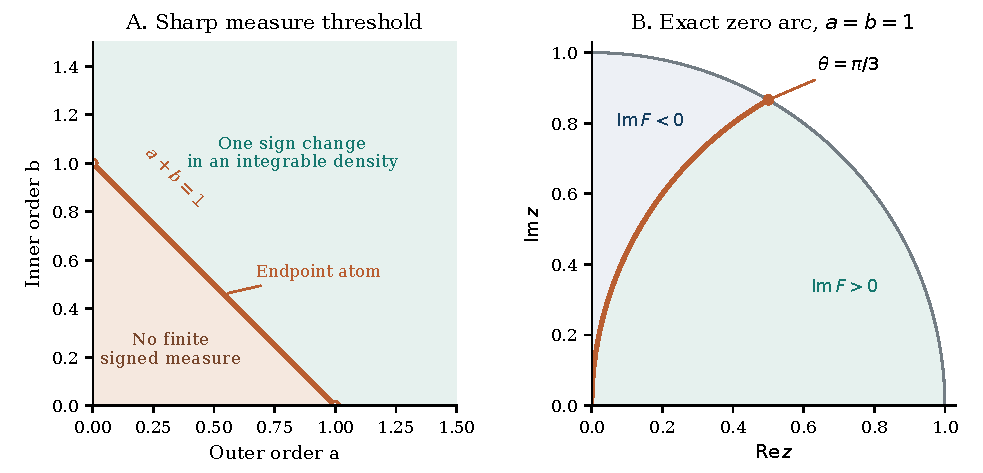
\includegraphics[width=\textwidth]{../figures/measure_geometry.pdf}
\caption{The sharp measure domain for positive real orders (left), and
an exact illustration of the angular-zero theorem in the first quadrant
at $a=b=1$ (right). The separating arc is $|1-z|=1$ and meets the
unit circle at angle $\pi/3$. The phase diagram is a theorem, and the
circular arc is evaluated exactly.}
\label{real:fig:geometry}
\end{figure}

\begin{corollary}[Continuous outer-order motion of the density crossing]
\label{real:cor:order-motion}
Fix $b>0$. If $a_2>a_1>0$ and $a_1+b>1$, then
$r_{a_2,b}<r_{a_1,b}$.
\end{corollary}
\begin{proof}
Put $\delta=a_2-a_1>0$. Multiplication of the moments by
$n^{-\delta}$ and uniqueness in Theorem~\ref{real:thm:measure}
give the Mellin-convolution formula
\[
 k_{a_2,b}(T)=\frac1{\Gamma(\delta)}
   \int_0^T(T-v)^{\delta-1}k_{a_1,b}(v)\,dv.
\]
Absolute exponential integrability justifies convolution and its
Laplace transform. Both sides are continuous for $T>0$, so moment
uniqueness gives pointwise equality. At the old logarithmic crossing
$T_1=-\log r_{a_1,b}$ the integrand is positive almost everywhere.
The new density is therefore positive at $T_1$, and its unique
crossing occurs at $T_2>T_1$. Returning to $r=e^{-T}$ proves the
claim.
\end{proof}

\subsection{Verification and the limits of the geometric conclusion}

The diagnostic program \path{code/geometry_diagnostics.py} and its
output \path{data/geometry_diagnostics.json} accompany these proofs.
They compare two kernel quadratures at nine points; locate four density
crossings, including $(a,b)=(0.5005,0.5)$ near the critical line; check
fifteen strictly negative critical-density values; and compute sixteen
interior-disk zero locations. The exact arc in
Example~\ref{real:ex:circle} supplies an independent comparator.
Twelve additional samples check the critical deficit and its first
four signed derivatives. All diagnostic assertions pass. The checks
are numerical and are not interval certificates; the existence,
uniqueness, and sign assertions rest on the analytic arguments above.

Near the critical line, direct subtraction of the two pieces of the
kernel can be unstable. For $0<a,b<1$ the evaluator instead uses
\[
 I(T)=q_T(1)\int_0^\infty c(s)\,ds
       +\int_0^\infty c(s)\bigl[q_T(s)-q_T(1)\bigr]\,ds,\qquad
 c(s)=g(s)/s.
\]
The first integral is the exact beta expression
\eqref{real:eq:beta}; the second integrand is negative on both
sides of $s=1$. At $a+b=1$ the beta term vanishes exactly. This is
the cancellation used in the proof, translated into a stable evaluator.

Three distinctions delimit the result. First,
$x_{a,b}'(R^2)>0$ does not by itself imply
$\theta_{a,b}'(R)<0$; that stronger angular monotonicity is not proved
here. Second, the monotone motion of the \emph{density} crossing with
$a$ does not imply monotone motion of the angular zero with $a$ or
$b$. Third, when $a+b<1$ the finite signed-measure method is
impossible by Theorem~\ref{real:thm:measure}, but this does not settle
zero uniqueness by other methods. The next section quantifies concentration into the endpoint atom
for fixed $b\in(0,1)$, providing a scale for uniform numerical evaluation.

\FloatBarrier
\section{The critical boundary: a power-law crossing and an exponential mass law}
\label{real:sec:boundary}

The atom in Theorem~\ref{real:thm:measure} raises a quantitative
question: how does an absolutely continuous positive part collapse into
that atom? Two distinct scales occur. Its outermost point approaches the
endpoint by a power of the distance to the critical line. Most of its
mass lies much closer to the endpoint, on an exponential scale described
by a limiting exponential distribution.

Fix $b\in(0,1)$, and write
\begin{equation}\label{real:eq:boundary-parameters}
 p=1-b,\qquad a=p+\varepsilon,\qquad
 k_\varepsilon(T)=k_{p+\varepsilon,b}(T),\qquad
 0<\varepsilon\leq\varepsilon_0<b.
\end{equation}
Let $T_\varepsilon$ be the unique logarithmic crossing of
$k_\varepsilon$, so $k_\varepsilon>0$ on $(0,T_\varepsilon)$.
All constants below may depend on the fixed $b$; the local expansion
constants may also depend on its chosen radius $T_0$.

\begin{lemma}[A uniform local kernel expansion]
\label{real:lem:boundary-expansion}
For any fixed $T_0<2\pi$, uniformly for
$0\leq\varepsilon\leq\varepsilon_0$ and $0<T\leq T_0$,
\begin{equation}\label{real:eq:boundary-expansion}
\begin{split}
 k_\varepsilon(T)=T^{\varepsilon-1}\biggl\{
 &\frac{\varepsilon}{p\Gamma(1+\varepsilon)}
 +\frac{\zeta(b)}{\Gamma(p+\varepsilon)}T^p
 -\frac{T}{2\Gamma(1+\varepsilon)}\\
 &-\frac{bT^2}{12\Gamma(2+\varepsilon)}+O_{b,T_0}(T^4)
 \biggr\}.
\end{split}
\end{equation}
More generally the bracket has the convergent expansion
\begin{equation}\label{real:eq:boundary-series}
\begin{split}
 &\frac{\varepsilon}{p\Gamma(1+\varepsilon)}
 +\frac{\zeta(b)}{\Gamma(p+\varepsilon)}T^p
 -\frac{T}{2\Gamma(1+\varepsilon)}\\
 &\hspace{8mm}
 -\sum_{\ell\geq1}\frac{B_{2\ell}\Gamma(b+2\ell-1)}
 {(2\ell)!\,\Gamma(b)\Gamma(\varepsilon+2\ell)}T^{2\ell},
 \qquad 0<T<2\pi.
\end{split}
\end{equation}
Here $B_{2\ell}$ are the Bernoulli numbers, with $B_2=1/6$.
\end{lemma}

\begin{proof}
Retain $g,I$ from \eqref{real:eq:scaled-integral}, now with
$a=p+\varepsilon$, and set
$h(v)=(e^v-1)^{-1}-v^{-1}$. Subtracting the leading singularity
inside the absolutely convergent integral gives the exact identity
\begin{equation}\label{real:eq:boundary-exact}
\begin{split}
 I(T)={}&\frac{J}{T}+\Gamma(b)\zeta(b)T^{-b}\\
 &-\int_0^1 s^{b-1}(1-s)^{a-1}h(Ts)\,ds,\qquad
 J=\frac{\varepsilon}{p}B(b,a).
\end{split}
\end{equation}
Indeed, $J=\int g(s)/s\,ds$ by \eqref{real:eq:beta}, and
\[
 \int_0^\infty s^{b-1}h(Ts)\,ds
 =T^{-b}\int_0^\infty v^{b-1}h(v)\,dv
 =\Gamma(b)\zeta(b)T^{-b}.
\]
The last integral converges for $0<b<1$. To identify it, subtract
$1/v$ from the Bose integral only on $(0,1)$ in the half-plane
$\Re b>1$ and continue the resulting expression to $\Re b>0$,
$b\ne1$. The added term is $1/(b-1)$. For $0<b<1$ it is exactly
$-\int_1^\infty v^{b-2}\,dv$, giving the displayed integral.
In particular $\zeta(b)<0$, since $h(v)<0$ for $v>0$.

Only a compact beta integral remains in
\eqref{real:eq:boundary-exact}. The convergent Taylor expansion
\[
 h(v)=-\frac12+\frac v{12}-\frac{v^3}{720}+\cdots,\qquad |v|<2\pi,
\]
may be integrated termwise there. For uniformity, choose a number
$T_1$ with $T_0<T_1<2\pi$. Cauchy's estimates on $|v|=T_1$
bound the Taylor remainders uniformly for $|v|\leq T_0$;
$s^{b-1}(1-s)^{p-1}$ dominates the beta weights for
$0\leq\varepsilon\leq\varepsilon_0$. Substituting the integrated
series into \eqref{real:eq:level} proves
\eqref{real:eq:boundary-series} and its stated uniform truncation.
\end{proof}

\begin{theorem}[Crossing scale and its first correction]
\label{real:thm:boundary-crossing}
Define
\begin{equation}\label{real:eq:tau}
 \tau_\varepsilon=
 \left\{\frac{\Gamma(p+\varepsilon)\varepsilon}
 {p[-\zeta(b)]\Gamma(1+\varepsilon)}\right\}^{1/p}.
\end{equation}
As $\varepsilon\downarrow0$,
\begin{equation}\label{real:eq:crossing-correction}
 T_\varepsilon
 =\tau_\varepsilon-\frac{\tau_\varepsilon^2}{2\varepsilon}
   +O_b\!\left(\frac{\tau_\varepsilon^3}{\varepsilon^2}\right).
\end{equation}
In particular, with
\begin{equation}\label{real:eq:boundary-constant}
 K_b=\left\{\frac{\Gamma(1-b)}{(1-b)[-\zeta(b)]}\right\}^{1/(1-b)},
\end{equation}
one has
\begin{equation}\label{real:eq:crossing-leading}
 T_\varepsilon\sim K_b\varepsilon^{1/(1-b)},\qquad
 1-r_{p+\varepsilon,b}\sim K_b\varepsilon^{1/(1-b)}.
\end{equation}
\end{theorem}

\begin{proof}
For every fixed $T>0$, the kernel depends continuously on
$\varepsilon$ and its limit $k_{p,b}(T)$ is strictly negative by
\eqref{real:eq:critical-density}. The unique crossing therefore
satisfies $T_\varepsilon\to0$. At that crossing, multiply the
bracket in \eqref{real:eq:boundary-expansion} by
$\Gamma(1+\varepsilon)$ and write
\[
 C_\varepsilon=
 \frac{[-\zeta(b)]\Gamma(1+\varepsilon)}{\Gamma(p+\varepsilon)}>0.
\]
This gives
\begin{equation}\label{real:eq:crossing-equation}
 \frac{\varepsilon}{p}
 =C_\varepsilon T_\varepsilon^p+
   \frac{T_\varepsilon}{2}
   +\frac{bT_\varepsilon^2}{12(1+\varepsilon)}
   +O_b(T_\varepsilon^4).
\end{equation}
Since $p<1$, the last three terms are lower order than
$T_\varepsilon^p$. Hence
$T_\varepsilon/\tau_\varepsilon\to1$.

Put $y=T_\varepsilon/\tau_\varepsilon$ and
$q=\tau_\varepsilon/\varepsilon$.
The leading equivalence implies $q=O_b(\varepsilon^{b/p})\to0$.
Dividing \eqref{real:eq:crossing-equation} by $\varepsilon/p$
gives, uniformly for $y$ near one,
\[
 1=y^p+\frac p2 qy+O_b(\varepsilon q^2).
\]
The mean value theorem first yields $y-1=O_b(q)$. Taylor expansion
then yields $p(y-1)+(p/2)q=O_b(q^2)$, so
$y=1-q/2+O_b(q^2)$. This proves
\eqref{real:eq:crossing-correction}. Formula
\eqref{real:eq:crossing-leading} follows from continuity of the
gamma factors and $1-e^{-T}\sim T$.
\end{proof}

At the symmetric boundary point $b=p=1/2$, the analytic correction
from the gamma quotient and the nonlinear root correction have the
same relative order. Using $\psi(1/2)=-\gamma-2\log2$ gives the
explicit consequence
\begin{equation}\label{real:eq:half-boundary}
\begin{split}
 T_\varepsilon={}&\frac{4\pi}{\zeta(1/2)^2}\varepsilon^2
 \left[1-
 \left(4\log2+\frac{2\pi}{\zeta(1/2)^2}\right)\varepsilon
 +O(\varepsilon^2)\right].
\end{split}
\end{equation}
For other $b$, retaining the exact gamma quotient in
$\tau_\varepsilon$ keeps the algebraic and fractional-power
corrections in \eqref{real:eq:crossing-correction} unambiguous.

\begin{theorem}[Condensation and the exponential positive-mass law]
\label{real:thm:boundary-mass}
Let $\mu_\varepsilon=\mu_{p+\varepsilon,b}$, and denote its positive
and negative parts by $\mu_\varepsilon^+$ and
$\mu_\varepsilon^-$, so $\mu_\varepsilon=
\mu_\varepsilon^+-\mu_\varepsilon^-$. Then
\begin{equation}\label{real:eq:boundary-measures}
 \mu_\varepsilon^-\longrightarrow
       -\kappa_{p,b}(u)\,du\quad\hbox{in total variation},\qquad
 \mu_\varepsilon^+\Longrightarrow\frac1p\delta_1.
\end{equation}
In particular $\mu_\varepsilon\Longrightarrow\mu_{p,b}$.

Let $\nu_\varepsilon$ be the pushforward of the finite positive
measure $p\,k_\varepsilon(T)^+e^{-T}\,dT$ under
$Y_\varepsilon=-\varepsilon\log T$. For all sufficiently small
$\varepsilon$ it is supported in $[0,\infty)$ and
\begin{equation}\label{real:eq:exponential-law}
 \left\|\nu_\varepsilon-e^{-y}\mathbf1_{y>0}\,dy
       \right\|_{\rm TV}
 =O_b\!\left(\varepsilon|\log\varepsilon|\right).
\end{equation}
The same convergence and rate hold after normalizing
$\nu_\varepsilon$ to a probability measure.
\end{theorem}

\begin{proof}
For $T\leq T_0<1$, Lemma~\ref{real:lem:boundary-expansion} gives
\begin{equation}\label{real:eq:boundary-leading-density}
 k_\varepsilon(T)=
 \frac{\varepsilon}{p\Gamma(1+\varepsilon)}T^{\varepsilon-1}
       +R_\varepsilon(T),\qquad
 |R_\varepsilon(T)|\leq C_bT^{p+\varepsilon-1}.
\end{equation}
The first term is positive, so the negative part is bounded by
$C_bT^{p-1}$, an integrable bound independent of $\varepsilon$.
For $T\geq T_0$, the scaled integral
\eqref{real:eq:scaled-integral} has a common integrable majorant as
$a$ ranges over $[p,p+\varepsilon_0]$; hence
$e^{-T}|k_\varepsilon(T)|\leq
C_be^{-T}(1+T^{\varepsilon_0})$. Pointwise convergence and dominated
convergence prove the negative-part assertion in
\eqref{real:eq:boundary-measures}. Its limiting mass is $1/p$ by
Theorem~\ref{real:thm:measure}. Each $\mu_\varepsilon$ has total
mass zero, so the positive masses have the same limit. Their supports
lie in $(e^{-T_\varepsilon},1)$, which shrinks to $1$; this proves
the positive weak limit.

For the quantitative distributional statement set
$y_\varepsilon=-\varepsilon\log T_\varepsilon$.
Theorem~\ref{real:thm:boundary-crossing} gives
$y_\varepsilon=O_b(\varepsilon|\log\varepsilon|)$ and
$y_\varepsilon>0$ for small $\varepsilon$.
On the positive support $0<T<T_\varepsilon$, replace the density
in \eqref{real:eq:boundary-leading-density} by its leading term
and replace $e^{-T}$ by one. The total variation error is at most
\[
 C_bT_\varepsilon^{p+\varepsilon}
     +C_b\varepsilon T_\varepsilon^{1+\varepsilon}
 =O_b(\varepsilon),
\]
because $T_\varepsilon^p=O_b(\varepsilon)$.
Total variation cannot increase under pushforward. With
$T=e^{-y/\varepsilon}$, the pushforward of the resulting leading
measure is exactly
\[
 \frac{e^{-y}}{\Gamma(1+\varepsilon)}
          \mathbf1_{y>y_\varepsilon}\,dy.
\]
Its total variation difference from the unit exponential density
is at most
$O(\varepsilon)+\int_0^{y_\varepsilon}e^{-y}\,dy$.
This proves \eqref{real:eq:exponential-law}. Its mass consequently
differs from one by the same order; normalizing changes the total
variation by at most that mass discrepancy.
\end{proof}

Thus the power-law crossing width does not describe the typical
positive-mass location. Under the normalized positive part,
$-\varepsilon\log(-\log u)$ tends to an exponential random variable
of mean one. A typical logarithmic distance $T=-\log u$ is therefore
exponentially small in $1/\varepsilon$, even though the outer edge of
the positive region is of order $\varepsilon^{1/(1-b)}$.

The accompanying boundary diagnostics compare the two-term root formula
at $b=1/4,1/2,3/4$ and decreasing $\varepsilon$, and compare positive-mass
distribution functions with the exponential law. The convergent series
\eqref{real:eq:boundary-series} provides a stable evaluator with a
recorded analytic truncation bound. Numerical rounding is still separate
from that bound; these are diagnostics, not new proof assumptions.

\begin{figure}[htbp]
\centering
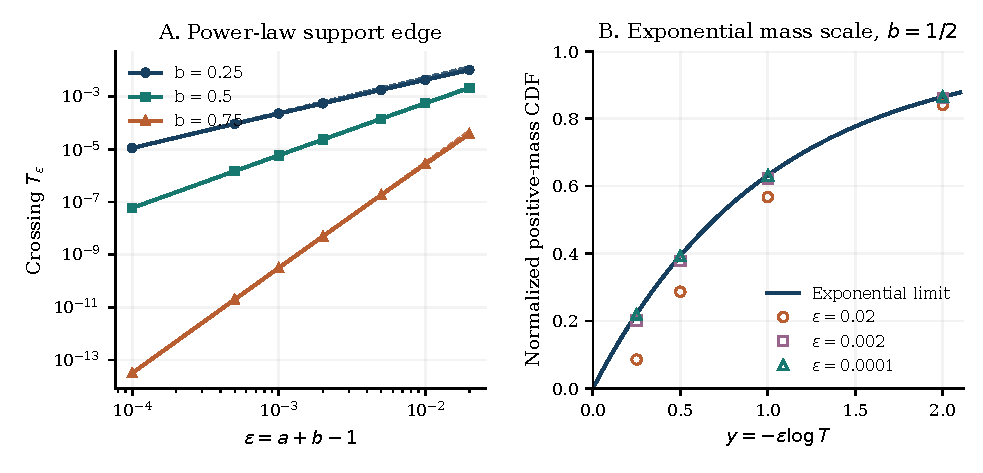
\includegraphics[width=\textwidth]{../figures/boundary_two_scales.pdf}
\caption{The two scales of endpoint concentration. Left: numerical
crossings (markers) and the leading power laws (dashed curves) at three
fixed inner orders. Right: four sampled distribution-function values
for each indicated $\varepsilon$ at $b=1/2$, compared with the proved
unit-exponential limit. These are diagnostics of the analytic results.}
\label{real:fig:boundary}
\end{figure}

All limits in this section keep $b$ fixed. As $b\downarrow0$, the
small parameter $\tau_\varepsilon/\varepsilon$ has exponent
$b/(1-b)\downarrow0$, so the stated hierarchy is not uniform at that
endpoint. As $b\uparrow1$, the exponent $1/(1-b)$ and the constants
become singular. Joint limits involving either endpoint require
additional analysis and are not consequences of these theorems.

\FloatBarrier
\section{A joint transition for reflected log-gamma moments}
\label{moment:sec}

The reflected family already considered in the manuscript is
\begin{equation}\label{moment:def}
 M_{n,m}=\int_0^1 f(x)^n f(1-x)^m\,dx,
 \qquad f(x)=\log\Gamma(x),\quad n,m\in\mathbb Z_{\ge0}.
\end{equation}
These mixed moments occur in Amdeberhan et al.~\cite[Section 5]{Amdeberhan2011}.
The manuscript proves that, for each fixed $m$,
\begin{equation}\label{moment:fixed}
 M_{n,m}\sim \frac{\gamma^m n!}{(m+1)^{n+1}},\qquad n\longrightarrow\infty,
\end{equation}
and develops the associated residues, late coefficients, and optimal truncation.
Its reflected-moment section explicitly leaves uniformity for growing $m$ open.
The result below identifies a transition where the leading expression
\eqref{moment:fixed} acquires a nontrivial factor. It concerns simultaneous
growth of the two exponents, rather than the late truncation index in the
already established fixed-$m$ expansion.

\subsection{The critical scale and the first correction}
Write $\gamma$ for Euler's constant, and define
\begin{equation}\label{moment:constants}
 c=\frac{\zeta(2)}{2\gamma}-\gamma,
 \qquad d=\frac{\zeta(3)}{3\gamma}
              -\frac{\zeta(2)^2}{8\gamma^2}.
\end{equation}
The constant $c$ is positive; for example $0<\gamma<0.6$ and
$\zeta(2)>1$ suffice to prove this. Its numerical value is
$c=0.8476712247576688767895678092\ldots$.
For $m\ge1$ put
\begin{equation}\label{moment:parameters}
 t=\frac{n}{m+1},\qquad \lambda=me^{-t},\qquad
 \mathcal R_{n,m}=\frac{(m+1)^{n+1}M_{n,m}}{\gamma^m n!}.
\end{equation}
All limits below are along integer pairs $(n,m)$ satisfying the stated
conditions. In particular $n>0$ and $t\ge2$ for all sufficiently large $m$.

\begin{theorem}[Uniform reflected-moment transition]\label{moment:thm:transition}
Fix $S>0$. Uniformly as $m\to\infty$ in the strip
$|t-\log m|\le S$, one has
\begin{equation}\label{moment:transition}
 \boxed{\displaystyle
 \mathcal R_{n,m}=e^{c\lambda}
 \left(1+\frac{C_1(t,\lambda)}m
              +O_S\!\left(\frac{t^2}{m^2}\right)\right),}
\end{equation}
where the correction is the explicit polynomial
\begin{equation}\label{moment:C1}
 C_1(t,\lambda)
 =\lambda\left[c\left(\frac t2-1\right)-2\gamma\right]
  +\lambda^2\left[\frac{c^2t}{2}+\gamma^2+d\right].
\end{equation}
Consequently, if $n/(m+1)-\log m\to s\in\mathbb R$, then
\begin{equation}\label{moment:profile}
 \mathcal R_{n,m}\longrightarrow \exp\!\left(c e^{-s}\right).
\end{equation}
\end{theorem}

For example, choosing $n$ to be the nearest integer to $(m+1)\log m$
gives $\mathcal R_{n,m}\to e^c=2.3342\ldots$, rather than $1$.
Thus the fixed-reflected-exponent leading term cannot be used uniformly
through this transition. The exact exponential in \eqref{moment:profile}
is more informative than a first-order correction to a fixed-$m$ formula.

\subsection{The exact probability representation}
Set
\[
 B(x)=\log\Gamma(1-x),\qquad \ell(x)=\log\Gamma(1+x).
\]
The standard expansions needed below are convergent for $|x|<1$
\cite[Section 5.7]{DLMF}:
\begin{align}\label{moment:endpoint-series}
 \ell(x)&=-\gamma x+\frac{\zeta(2)}2x^2
                    -\frac{\zeta(3)}3x^3+\cdots,\notag\\
 B(x)&=\gamma x+\frac{\zeta(2)}2x^2
                    +\frac{\zeta(3)}3x^3+\cdots.
\end{align}
The inequality $\psi'(x)>0$, together with $\psi(1)=-\gamma<0$,
shows that $f(x)>0$ on $(0,1)$. Log-convexity of $\Gamma$ between $1$
and $2$ gives $\ell(x)\le0$, hence
\begin{equation}\label{moment:elementary-bound}
 0<f(x)\le-\log x\quad(0<x<1),\qquad
 \int_0^1 f(x)^m\,dx\le m!.
\end{equation}

Let $r=m+1$ and let $Y$ have the gamma density with shape $n+1$ and rate $r$:
\[
 p(y)=\frac{r^{n+1}}{n!}y^n e^{-ry},\qquad y>0.
\]
Its mode is exactly $t=n/r$. The substitution $x=e^{-y}$ in
\eqref{moment:def} gives the identity
\begin{equation}\label{moment:expectation}
 \mathcal R_{n,m}=\mathbb E\,e^{E_m(Y)},
\end{equation}
where
\begin{equation}\label{moment:weight}
 E_m(y)=n\log\left(1+\frac{\ell(e^{-y})}{y}\right)
       +m\log\left(\frac{B(e^{-y})}{\gamma e^{-y}}\right).
\end{equation}
The expressions inside both logarithms are positive for $y>0$.
Equation \eqref{moment:expectation} is exact, with no asymptotic interchange.

\subsection{Why the weighted tails are negligible}
Ordinary gamma concentration is not by itself sufficient in
\eqref{moment:expectation}: the multiplying weight can grow on the left.
We therefore prove the required estimate explicitly.

\begin{lemma}[Uniform weighted localization]\label{moment:lem:localization}
For each fixed $S>0$, there are positive constants $C_S,c_S$ such that,
for all sufficiently large $m$ with $|t-\log m|\le S$,
\begin{equation}\label{moment:localization}
 \mathbb E\left[e^{E_m(Y)}\mathbf1_{\{|Y-t|>1\}}\right]
 \le C_S\exp\!\left(-c_S\frac m t\right).
\end{equation}
Unweighted tails with any fixed polynomial factor in $|Y-t|$ obey the
same type of bound, after altering the constants.
\end{lemma}

\begin{proof}
Let $y_0=\log2$. For $0<x\le1/2$, positivity of the coefficients of $B$
and $\zeta(j)/j\le\zeta(2)/2$ for $j\ge2$ give
\[
 \frac{B(x)}{\gamma x}
 \le1+\frac{\zeta(2)x}{2\gamma(1-x)}
 \le1+C x,\qquad C=\frac{\zeta(2)}\gamma.
\]
Since $\ell\le0$, this implies
\begin{equation}\label{moment:weight-bound}
 e^{E_m(y)}\le \exp(Cme^{-y}),\qquad y\ge y_0.
\end{equation}

On $0<y<y_0$, use the original moment integral and
\eqref{moment:elementary-bound}. The unnormalized contribution is at most
$y_0^n m!$. Stirling's bounds show that the logarithm of its normalized
contribution is
\[
 -n\log t+O_S(n+m\log m).
\]
In the strip, $m\log m=O_S(n)$, so this is at most
$-\tfrac12n\log t$ for sufficiently large $m$.

On $y_0\le y\le t/2$, the weight is at most $e^{Cm/2}$.
The gamma lower-tail bound at half the mode is $e^{-c_0n}$ for a fixed
$c_0>0$ once $n$ is large. This follows directly from the moment-generating
function $(1-u/r)^{-n-1}$ and exponential Markov inequality.
Since $n/m\sim\log m$, the weighted contribution is $O(e^{-c_1mt})$.

On $t/2\le y\le t-1$, write $u=t-y$. The exact ratio to the density at
the mode satisfies
\begin{equation}\label{moment:density-ratio}
 \frac{p(t-u)}{p(t)}
 =\exp\{n\log(1-u/t)+ru\}
 \le\exp\!\left(-\frac{ru^2}{2t}\right).
\end{equation}
The weight in \eqref{moment:weight-bound} is at most $\exp(C\lambda e^u)$.
For $1\le u\le t/2$, the maximum of $e^u/u^2$ occurs at an endpoint.
As $\lambda\in[e^{-S},e^S]$ and $t=\log m+O_S(1)$, it follows that
\[
 C\lambda e^u\le \frac{ru^2}{4t}
\]
uniformly on this interval when $m$ is large. Multiplication by
\eqref{moment:density-ratio}, followed by integration and
$p(t)=O(\sqrt{r/t})$, gives $O_S(e^{-c_2m/t})$.

Finally, on $y\ge t+1$, the weight is bounded by $\exp(C\lambda/e)$.
The gamma upper-tail bound for a displacement of one from the mode is
$O_S(e^{-c_3m/t})$. For completeness, with mean $(n+1)/r=t+1/r$,
the usual gamma exponent at $t+1$ is
$(n+1)(\delta-\log(1+\delta))$, where
$\delta=(r-1)/(n+1)\asymp1/t$; this exponent is bounded below by a
positive constant times $r/t$.
The four estimates prove \eqref{moment:localization}. Inserting a fixed
polynomial in the tails only introduces polynomial factors, which can
be absorbed by reducing the positive exponential constant. The density
ratio or the same exponential Markov argument gives this last assertion.
\end{proof}

\subsection{Proof of the transition and its explicit correction}
\begin{proof}[Proof of Theorem~\ref{moment:thm:transition}]
For the calculation abbreviate
\[
 a=-\gamma,\quad a_2=\zeta(2)/2,\quad b=\zeta(2)/(2\gamma),
 \quad c=a+b.
\]
Let $V=Y-t$. Uniformly for $|v|\le1$, set
$x=(\lambda/m)e^{-v}$ and use \eqref{moment:endpoint-series} with its
analytic remainder. One obtains
\begin{equation}\label{moment:local-expansion}
 E_m(t+v)=A(v)+\frac{B_1(v)}m+O_S(m^{-2}),
\end{equation}
where
\begin{align}\label{moment:local-functions}
 A(v)&=\lambda e^{-v}\left(b+\frac{at}{t+v}\right),\notag\\
 B_1(v)&=\frac{a\lambda te^{-v}}{t+v}
 +\lambda^2e^{-2v}\left(d+\frac{a_2t}{t+v}
                            -\frac{a^2t}{2(t+v)^2}\right).
\end{align}
All derivatives of each fixed order used below are uniformly bounded
in this interval; $t/(t+v)$ is bounded once $t\ge2$.

The exact moments about the mode, rather than about the mean, are
\begin{align}\label{moment:central-moments}
 \mathbb EV&=r^{-1},&
 \mathbb EV^2&=t/r+2/r^2,\notag\\
 \mathbb EV^3&=5t/r^2+6/r^3,&
 \mathbb EV^4&=3t^2/r^2+26t/r^3+24/r^4.
\end{align}
They follow either from gamma raw moments or from
$\mathbb Ee^{zV}=e^{-tz}(1-z/r)^{-rt-1}$.
Taylor expand $e^{A(v)}$ through degree three and bound its fourth
remainder with \eqref{moment:central-moments}. The cubic term is
$O_S(t/m^2)$ because its signed moment, not its absolute third moment,
is used. Expand $e^{A(v)}B_1(v)$ through degree one with a quadratic
remainder. Lemma~\ref{moment:lem:localization} allows us to use full
gamma moments and discard the outer tails. The result is
\begin{align}\label{moment:first-reduction}
 e^{-A(0)}\mathcal R_{n,m}
 =1+\frac1m\left[B_1(0)+A'(0)
       +\frac t2\{A''(0)+A'(0)^2\}\right]
 +O_S(t^2/m^2).
\end{align}
Here replacing $r^{-1}$ by $m^{-1}$ changes only the stated remainder.

The local values are
\begin{align*}
 A(0)&=c\lambda,& A'(0)&=-\lambda(c+a/t),\\
 A''(0)&=\lambda(c+2a/t+2a/t^2),&
 B_1(0)&=a\lambda+\lambda^2(d+a_2-a^2/(2t)).
\end{align*}
Substitution into \eqref{moment:first-reduction} cancels all negative
powers of $t$ and yields
\[
 \lambda\{c(t/2-1)+2a\}
 +\lambda^2\{c^2t/2+ca+d+a_2\}.
\]
The relation $ca+a_2=\gamma^2$ gives \eqref{moment:C1}.
Since $t/m\to0$, the limit \eqref{moment:profile} follows immediately.
\end{proof}

\subsection{All fixed asymptotic orders}
\begin{theorem}[Constructive expansion to every fixed order]
\label{moment:thm:all-orders}
For each integer $J\ge0$, there are explicitly computable functions
$C_j(t,\lambda)$, polynomial in $\lambda$ and rational in $t$, such that
$C_0=1$, $C_1$ is \eqref{moment:C1}, and
\begin{equation}\label{moment:all-orders}
 \mathcal R_{n,m}=e^{c\lambda}
 \left[\sum_{j=0}^J\frac{C_j(t,\lambda)}{m^j}
 +O_{S,J}\!\left(\frac{t^{J+1}}{m^{J+1}}\right)\right]
\end{equation}
uniformly in $|t-\log m|\le S$. For each fixed $j$,
$C_j(t,\lambda)=O_{S,j}(t^j)$. The theorem asserts an expansion at every
fixed order, without asserting convergence of the infinite expansion.
\end{theorem}

The following finite differential prescription makes ``computable''
precise. Let $\epsilon$ be a formal variable and put
$r=(1+\epsilon)/\epsilon$. Define
\begin{align}\label{moment:formal-Phi}
 \Phi_\epsilon(v)=\epsilon^{-1}\Bigg[
 &(1+\epsilon)t\log\left(1+
 \frac{\ell(\lambda\epsilon e^{-v})}{t+v}\right)\notag\\
 &+\log\left(\frac{B(\lambda\epsilon e^{-v})}
                        {\gamma\lambda\epsilon e^{-v}}\right)\Bigg],\\
 K_\epsilon(z)&=\frac zr+
 \sum_{k\ge2}\left(\frac{t}{kr^{k-1}}+
                         \frac1{kr^k}\right)z^k.
 \label{moment:formal-K}
\end{align}
The quotient involving $B$ has constant term one, and both terms in
brackets vanish at $\epsilon=0$, so the formal expression is well defined.
With derivatives acting on $v$, the coefficients are
\begin{equation}\label{moment:coefficient-algorithm}
 C_j(t,\lambda)=e^{-c\lambda}[\epsilon^j]
 \left.\exp\!\bigl(K_\epsilon(\partial_v)\bigr)
                      e^{\Phi_\epsilon(v)}\right|_{v=0}.
\end{equation}
Only finitely many derivatives occur at a fixed order: the maximum
derivative order at $\epsilon^j$ is $2j$.

\begin{proof}[Proof of Theorem~\ref{moment:thm:all-orders}]
Expand \eqref{moment:weight} through order $J$ in $1/m$ on $|v|\le1$.
The convergent endpoint series make its remainder, together with any
fixed number of $v$ derivatives, uniformly $O_{S,J}(m^{-J-1})$.
Expand the resulting analytic amplitudes in $v$ through degree $2J+1$.
Gamma moment--cumulant identities give
\[
 \mathbb E|V|^{2J+2}=O_J\!\left((t/m)^{J+1}\right),
\]
while signed odd moments occur at integer powers of $1/m$ and have the
corresponding smaller order. These facts follow directly by expanding
the exact logarithm of the moment-generating function, which is
\eqref{moment:formal-K}. Lemma~\ref{moment:lem:localization} controls
the tails, including every polynomial moment used here.
Taylor's theorem therefore gives \eqref{moment:all-orders} with the
displayed remainder.

At each fixed order all derivatives at $v=0$ of
$t/(t+v)$ are rational functions of $t$, and all endpoint coefficients
are finite combinations of $\gamma$ and zeta values. The common
exponential factor is $e^{c\lambda}$. This proves the stated coefficient
class and \eqref{moment:coefficient-algorithm}. At formal order $j$, the
moment--cumulant formula introduces at most $j$ positive powers of $t$;
the remaining amplitude derivatives are bounded as $t\to\infty$.
Consequently $C_j=O_{S,j}(t^j)$.
\end{proof}

For a compact reproducible second-order formula, retain $a=-\gamma$,
$a_2=\zeta(2)/2$ and let
$\alpha_j=A^{(j)}(0)$ and $\beta_j=B_1^{(j)}(0)$, using
\eqref{moment:local-functions}. Put
\[
 a_3=-\zeta(3)/3,\qquad
 e=\frac{\zeta(4)}{4\gamma}
       -\frac{\zeta(2)\zeta(3)}{6\gamma^2}
       +\frac{\zeta(2)^3}{24\gamma^3},
\]
and
\begin{align*}
 D_0={}&\lambda^2\left(a_2-\frac{a^2}{2t}\right)
       +\lambda^3\left(e+a_3-\frac{aa_2}{t}
                               +\frac{a^3}{3t^2}\right),\\
 R_2={}&\alpha_2+\alpha_1^2,\qquad
 R_3=\alpha_3+3\alpha_1\alpha_2+\alpha_1^3,\\
 R_4={}&\alpha_4+4\alpha_1\alpha_3+3\alpha_2^2+6\alpha_1^2\alpha_2+\alpha_1^4.
\end{align*}
Then the exact formula generated by \eqref{moment:coefficient-algorithm} is
\begin{align}\label{moment:C2}
 C_2={}&D_0+\tfrac12 \beta_0^2+\beta_1+\alpha_1\beta_0
       +\tfrac t2(\beta_2+2\alpha_1\beta_1+R_2\beta_0)\notag\\
       &-\alpha_1+\tfrac{2-t}{2}R_2+\tfrac{5t}{6}R_3+\tfrac{t^2}{8}R_4.
\end{align}
The accompanying symbolic program expands \eqref{moment:C2} into a
polynomial of degree at most two in $t$ and four in $\lambda$ and checks
the first-correction cancellation by exact algebra.

\subsection{Exact identities for diagonals of the residue array}
The existing meromorphic moment transform has residues determined by
\begin{equation}\label{moment:residues}
 A_{k,m}=\frac1k[x^{k-1}]\Gamma(1+x)^k B(x)^m.
\end{equation}
The joint transition has an exact algebraic counterpart in their
near-diagonal coefficients.

\begin{proposition}[Diagonal residue polynomials]\label{moment:prop:diagonals}
Put
\[
 P_j(m)=(m+j+1)\gamma^{-m}A_{m+j+1,m},\qquad
 H(x)=\frac{\Gamma(1+x)B(x)}{\gamma x}.
\]
Then $P_j$ is a polynomial in $m$ of degree $j$, with leading coefficient
$c^j/j!$, and
\begin{equation}\label{moment:diagonal}
 P_j(m)=[x^j]\Gamma(1+x)^{j+1}H(x)^m.
\end{equation}
Write $\ell_r=[x^r]\ell(x)$ and $h_r=[x^r]\log H(x)$. An explicit
finite identity is
\begin{equation}\label{moment:partition}
 P_j(m)=\sum_{\nu_1+2\nu_2+\cdots+j\nu_j=j}
       \prod_{r=1}^j\frac{(mh_r+(j+1)\ell_r)^{\nu_r}}{\nu_r!}.
\end{equation}
In particular,
\begin{align}\label{moment:first-P}
 P_0(m)&=1,\qquad P_1(m)=mc-2\gamma,\notag\\
 P_2(m)&=\tfrac12m^2c^2
       +m\{\zeta(2)/2+d-3\gamma c\}
       +\tfrac32\zeta(2)+\tfrac92\gamma^2.
\end{align}
If $g(w)$ is the inverse germ of $x/\Gamma(1+x)$, then
\begin{equation}\label{moment:diagonal-generator}
 \sum_{j\ge0}P_j(m)w^j
 =g'(w)\left(\frac{B(g(w))}{\gamma w}\right)^m.
\end{equation}
These identities are identities of formal power series, with no
assertion about convergence of the divergent full moment pole expansion.
\end{proposition}

\begin{proof}
Insert $k=m+j+1$ in \eqref{moment:residues} and remove the factor
$(\gamma x)^m$. This proves \eqref{moment:diagonal}.
Expansion of the exponential of
$m\log H(x)+(j+1)\ell(x)$ proves \eqref{moment:partition}.
The coefficient of $x$ in $\log H$ is $c>0$, so the leading coefficient
in $m$ is exactly $c^j/j!$. The first two further coefficients yield
\eqref{moment:first-P}.

Let $W_m(x)=\int_0^x B(u)^m\,du$. Lagrange--B\"urmann inversion gives
\[
 W_m(g(w))=\sum_{k\ge1}A_{k,m}w^k.
\]
Differentiate and divide by $\gamma^m w^m$. The result is precisely
\eqref{moment:diagonal-generator}.
\end{proof}

For fixed $j$, the contribution of the residue at $m+j+1$, normalized
by the leading scale in \eqref{moment:fixed}, is
\[
 P_j(m)\left(\frac{m+1}{m+j+1}\right)^{n+1}
 =\frac{(c\lambda)^j}{j!}+O_{S,j}(t/m).
\]
The exponential profile is therefore the natural resummation of the
near-diagonal residue directions. This observation explains the answer;
the weighted integral proof above is what justifies the uniform limit.
It would be invalid to obtain that limit by simply summing the divergent
infinite fixed-$m$ pole expansion.

\subsection{Numerical diagnostics}
The two numerical implementations in the package integrate respectively
in $y=-\log x$ and directly in $x$, splitting at the moving saddle.
They agree to the working precision of 60 decimal digits in the eight
recorded cases. The calculations are high-precision diagnostics, not
rational or interval enclosures. The analytic proofs establish the error orders.
Table~\ref{moment:tab} records the central transition sequence; rounding
of $n$ is incorporated in the actual $t$ and $\lambda$ in each formula.

\begin{table}[htbp]
\centering\small
\begin{tabular}{rrrrr}
\toprule
$m$&$n$&$\mathcal R_{n,m}$&Error after $C_1$&Error after $C_2$\\
\midrule
30&105&2.427573439030&$1.0791\cdot10^{-2}$&$3.9071\cdot10^{-3}$\\
100&465&2.376317091692&$1.8754\cdot10^{-3}$&$2.0084\cdot10^{-4}$\\
300&1717&2.352781323812&$3.9099\cdot10^{-4}$&$1.4153\cdot10^{-5}$\\
1000&6915&2.341576352534&$6.1750\cdot10^{-5}$&$7.4413\cdot10^{-7}$\\
\bottomrule
\end{tabular}
\caption{Numerical diagnostics for $n$ nearest to $(m+1)\log m$.
Errors are the computed ratio minus the indicated approximation.
No monotone improvement for every parameter and truncation is asserted.}
\label{moment:tab}
\end{table}

\begin{figure}[htbp]
\centering
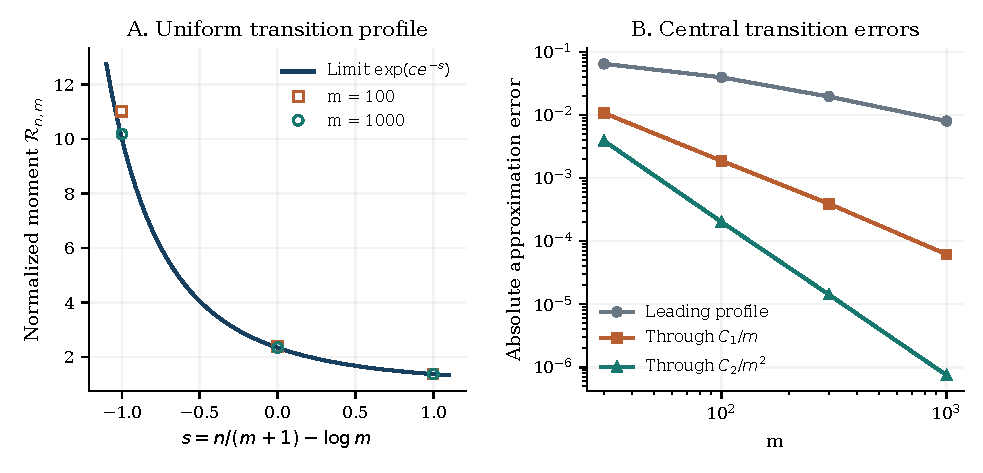
\includegraphics[width=\textwidth]{../figures/moment_transition.pdf}
\caption{The proved profile $\exp(c e^{-s})$ and numerical checks near
the central transition. The second panel shows errors of the successive
approximations along the four cases in Table~\ref{moment:tab}. The curves
visualize the theorem and its diagnostics; they supply no independent proof.}
\label{moment:fig}
\end{figure}

\FloatBarrier
\section{A sharp formal obstruction at weight six}
\label{depthnew:sec:obstruction}

The audited manuscript proves a complementary-depth bound for one-variable
multiple polylogarithms: after adjoining a transformed argument and endpoint
constants, a weight-$w$, depth-$d$ value has a representation of reduced
depth at most $w-d$. The first critical triple weight is therefore six.
The following result identifies exactly what survives if one tries to
reduce every such triple further using shuffle products and the six
standard argument transformations. It is a theorem about a specified
formal quotient, with no assertion of numerical period independence.

\subsection{The quotient and the argument action}

Let $V=\mathbb Qx+\mathbb Qy$, let $\operatorname{Sh}(V)$ be its shuffle
algebra, and let $J$ be the augmentation ideal. Set
\[
 Q_6=(J/J^2)_6.
\]
The depth of a binary word is its number of $y$ letters. Including words
with trailing $x$ makes linear substitutions immediate; shuffle
normalization with $H_x(z)=\log z$ removes such trailing letters without
changing the positive-weight indecomposable quotient.
The usual outer-letter-first interpretation is
\[
 x=\frac{dt}{t},\qquad y=\frac{dt}{1-t},\qquad
 H_{0^{s_1-1}1\cdots0^{s_d-1}1}(z)
 =\Li_{s_1,\ldots,s_d}(z,1,\ldots,1),
\]
where $0$ denotes $x$ and $1$ denotes $y$.

The group of six M\"obius transformations permuting $0,1,\infty$ acts
on the letter space through the matrices
\begin{equation}\label{depthnew:eq:matrices}
 R=\begin{pmatrix}0&-1\\-1&0\end{pmatrix},\qquad
 M=\begin{pmatrix}1&0\\1&-1\end{pmatrix}.
\end{equation}
Matrices act on columns, so $R(x)=-y$, $R(y)=-x$, whereas
$M(x)=x+y$, $M(y)=-y$. These are the pullbacks for $z\mapsto1-z$
and $z\mapsto z/(z-1)$, respectively. The six matrices are
$I,R,M,RM,MR,RMR$.
Landen substitution fixes the initial endpoint zero. Complementation
changes it to one; ordinary path composition supplies endpoint constants
and products of lower-weight integrals. Thus the same letter action
models these argument changes modulo products and endpoint constants.
The formal space is defined independently of any special-point evaluation.

\begin{theorem}[Exactly one missing triple direction]
\label{depthnew:thm:codimension}
Let $D_2\subset Q_6$ be the span of words of depth at most two, and
let $E_2$ be the span of their images under the six matrices above. Then
\[
 \dim Q_6=9,\qquad \dim E_2=8.
\]
The span is unchanged if all of $\operatorname{GL}_2(\mathbb Q)$ is
allowed in place of the six matrices. Its annihilator is generated by
coefficient pairing with the Lie polynomial
\begin{equation}\label{depthnew:eq:omega}
 \Omega=\bigl[[x,[x,y]],[y,[x,y]]\bigr].
\end{equation}
On the three triple generators used in the manuscript this pairing is
\begin{equation}\label{depthnew:eq:triple-values}
\begin{array}{c|ccc}
\text{word}&000111&001011&001101\\
\text{index}&(4,1,1)&(3,2,1)&(3,1,2)\\ \hline
\langle\Omega,\text{word}\rangle&0&-1&2.
\end{array}
\end{equation}
In particular, the class of $(3,2,1)$ supplies the single additional
formal direction.
\end{theorem}

\begin{proof}
The coefficient pairing is
$\langle\sum a_ww,\sum b_ww\rangle=\sum a_wb_w$.
Lie polynomials are primitive for the coproduct dual to shuffle
multiplication: this follows from
$\Delta x=x\otimes1+1\otimes x$, the same formula for $y$, and closure
of primitive elements under commutators. Hence every Lie polynomial
pairs to zero with every shuffle product of two nonempty words.
Consequently $\Omega$ defines a functional on $Q_6$.

Every word in $\Omega$ has exactly three $x$ and three $y$ letters,
so the functional vanishes on $D_2$. It is nonzero: the coefficient
of $001011$ is $-1$, and expansion gives the three entries in
\eqref{depthnew:eq:triple-values}.
There is also a covariance under every invertible linear substitution
$N$. Put $C=[x,y]$, $A=[x,C]$, and $B=[y,C]$.
The element $C$ transforms by $\det N$, while the pair $(A,B)$
transforms by $\det N$ times the original two-dimensional matrix.
Their commutator therefore satisfies
\begin{equation}\label{depthnew:eq:covariance}
 N(\Omega)=(\det N)^3\Omega.
\end{equation}
Since $N$ and its transpose have the same determinant,
\[
 \langle\Omega,N(w)\rangle
 =\langle N^{\mathsf T}(\Omega),w\rangle
 =(\det N)^3\langle\Omega,w\rangle.
\]
Thus $\Omega$ annihilates the full linear-letter orbit of $D_2$.
Both proposed spans have codimension at least one.

For the reverse inequality, the Lyndon description of the shuffle
algebra \cite{depthnew:Radford} gives the binary Witt count
\[
 \dim Q_6=\frac{2^6-2^3-2^2+2}{6}=9.
\]
The nine Lyndon words are
\[
\begin{gathered}
000001,\ 000011,\ 000101,\ 000111,\ 001011,\ 001101,\\
001111,\ 010111,\ 011111.
\end{gathered}
\]
For each Lyndon word $l$, let $b(l)$ denote its standard Lie bracketing:
if $l=uv$ and $v$ is its longest proper Lyndon suffix, put
$b(l)=[b(u),b(v)]$, with the letters as initial cases.
These nine primitive elements form a dual family of functionals on $Q_6$.

Take, in order, the eight word classes
\[
\begin{gathered}
 I(000001),\ I(000011),\ I(000101),\\
 R(000001),\ R(000011),\ R(000101),\\
 M(000001),\ M(000101),
\end{gathered}
\]
and pair them with the eight $b(l)$ obtained by omitting $001101$
from the ordered Lyndon list. Direct commutator expansion gives
\begin{equation}\label{depthnew:eq:minor}
\begin{pmatrix}
 1& 0& 0& 0& 0& 0& 0& 0\\
 0& 1& 0& 0& 0& 0& 0& 0\\
 0&-2& 1& 0& 0& 0& 0& 0\\
 0& 0& 0& 0& 0& 0& 0&-1\\
 0& 0& 0& 0& 0&-1& 0& 0\\
 0& 0& 0& 0& 0& 4&-1& 0\\
-1& 1& 0&-1& 0& 1& 0&-1\\
 0&-2& 1& 4& 1&-7&-1&11
\end{pmatrix}.
\end{equation}
Its determinant is $1$, proving independence of the eight classes.
The six-transformation span is consequently the eight-dimensional
kernel of $\Omega$. The full linear-letter span lies between that
space and the same kernel, proving the stronger assertion too.
\end{proof}

\subsection{Two exact quotient identities}

The rank statement also supplies concise constructive reductions.
Write $F_{a,b}(z)=\Li_{a,b}(z,1)$ and
$F_{a,b,c}(z)=\Li_{a,b,c}(z,1,1)$, and put
$u=1-z$, $v=z/(z-1)$.
Here $\equiv$ denotes equality modulo products of positive-weight
hyperlogarithms and endpoint constants, of total weight six.
The identities use the common analytic continuation from $0<z<1$.

\begin{proposition}\label{depthnew:prop:congruences}
One has
\begin{align}
 F_{4,1,1}(z)\equiv{}&-\Li_6(z)+F_{5,1}(z)
 +\Li_6(u)-F_{5,1}(u)-\Li_6(v),
 \label{depthnew:eq:411}\\
 2F_{3,2,1}(z)+F_{3,1,2}(z)\equiv{}&
 -\Li_6(z)+F_{5,1}(z)+F_{4,2}(z)\notag\\
 &-10\Li_6(u)+10F_{5,1}(u)+F_{4,2}(u)\notag\\
 &-\Li_6(v)-F_{4,2}(v).
 \label{depthnew:eq:321312}
\end{align}
\end{proposition}
\begin{proof}
Expand the nine rows obtained by applying $I,R,M$, in that order,
to $000001,000011,000101$.
The coefficient vectors for \eqref{depthnew:eq:411} and
\eqref{depthnew:eq:321312}, respectively, are
\[
 (-1,1,0,1,-1,0,-1,0,0),\qquad
 (-1,1,1,-10,10,1,-1,0,-1).
\]
Subtract each corresponding word combination from its left side.
Pairing the residual with each of the nine standard Lyndon Lie
polynomials gives zero, by direct expansion. The primitive space is dual
to the indecomposable quotient, so each residual belongs to $J^2$.
Landen pullback and the endpoint-transport formula then give the stated
analytic congruences. This is an equality in the specified quotient;
no product term is silently asserted to vanish as a function.
\end{proof}

The supplied standard-library verifier reconstructs all of these objects,
checks the determinant-one minor, verifies the two congruences, and
checks $\Omega$ against all $320$ nonempty binary shuffle products of
weight six. Every operation uses exact integers or rational numbers.
No numerical polylogarithm value or rank estimate enters.

\paragraph{Consequences and limits.}
The general complementary-depth bound three is sharp for this formal
class at weight six, even after the argument alphabet is enlarged by
all six standard transformations. Exactly one triple coordinate remains,
rather than an unspecified failure of a search.
At a particular cyclotomic point, additional identities can still kill
that coordinate. The theorem therefore proves neither numerical
irreducibility of $F_{3,2,1}(i)$ nor an obstruction to identities using
other color alphabets. The existing octahedral $S_4$ proof illustrates
why enlarging the available laws can overcome a restricted formal
obstruction. The manuscript's $S_6$ candidate remains conjectural.

\section{Corrections and status revisions for the manuscript}
\label{editorial:sec}
The source's discovery chapter already gives a careful distinction
between experimental evidence, exact relation matrices, and numerical
period identities. A few earlier passages should be brought into line
with that standard. The proposed patch is restricted to the pinned
source and is supplied for review; it has not been applied to the
remote repository.

\subsection{A definite bibliographic correction}
The plastic-base discussion in
\path{chapters/03-algebraic.tex} describes a sequel of
Abouzahra--Lewin as never published. The sequel was published:
M.~Abouzahra, L.~Lewin, and Xiao Hongnian,
\emph{Polylogarithms in the field of omega (a root of a given cubic):
Functional equations and ladders},
\emph{Aequationes Mathematicae} \textbf{33} (1987), 23--45
\cite{AbouzahraLewinXiao1987}.
The publisher records the issue date as February 1987 and the DOI as
\texttt{10.1007/BF01836149}.
Its abstract distinguishes analytically derived lower-order results
from numerically found higher-order ladders. Restoring this reference
therefore improves both attribution and proof-status tracking.

The later literature also includes Gangl's functional equations and
proved ladders in weights six and seven \cite{Gangl2013}.
Those statements use a single-valued modified polylogarithm; the
projection is the real part in odd weight and the imaginary part in
even weight. In particular, an even-weight modified identity at real
arguments cannot simply be read as an identity for ordinary real
\(\Li_{2k}\). The correction patch makes this normalization distinction
explicit.

\subsection{Numerical confirmation is a distinct status}
The golden-ladder discussion uses headings and phrases such as
\emph{conjectures, verified}, \emph{also hold}, and \emph{are correct}
beside finite-precision residual checks. A small computed residual
establishes numerical consistency with a formula. By itself it does
not establish an identity of periods. The proposed edits say
\emph{numerically confirmed} where that is the evidence actually
provided, and retain analytic or exact status when a proof is present.

This is a local editorial correction, not a claim that every displayed
historical ladder lacks a proof in the literature. A formula with a
published proof should be matched to that proof, including its
normalization and branches. A proposed specialization of a functional
equation should include the exact substitution and residual
cancellation. In particular, citing a family of Kummer equations
without supplying or identifying the required specialization is less
specific than a replayable derivation.

The new seed theorem sharpens the source's support question but does
not remove this distinction. It proves that no new positive even
golden power adds a multiplicative seed. It does not prove the
constants in each higher ladder or a maximal ladder weight of nine.
The remaining question concerns compatibility with functional equations,
products, and regulator data on an already complete seed space.

\subsection{Restoring a missing canonical ladder definition}
The canonical elimination chain in the same source uses \(L_{12}\)
without defining it. Its logarithmic tail also contains factorials
with negative indices at the low orders where vanishing is discussed.
The proposed repair omits those summands and reconstructs the missing
notation from the first displayed weight-five formula.
Put \(\ell=\log\rho\) and, for \(n\ge1\), define
\begin{align}
 \mathrm{tw}_{12}(n)={}&-\frac{13}{48}\frac{\ell^n}{n!}
 +\frac1{48}\zeta(2)\frac{\ell^{n-2}}{(n-2)!}
 -\frac{19}{1728}\zeta(4)\frac{\ell^{n-4}}{(n-4)!},
 \label{editorial:eq:tail}\\
 L_{12}(n)={}&\frac{\Li_n(\rho^{12})}{12^{n-1}}
 -\frac32\frac{\Li_n(\rho^6)}{6^{n-1}}
 -\frac{\Li_n(\rho^4)}{4^{n-1}}
 +\frac{11}{48}\frac{\Li_n(\rho^2)}{2^{n-1}}
 +\mathrm{tw}_{12}(n).
 \label{editorial:eq:L12}
\end{align}
The negative-factorial convention applies in \eqref{editorial:eq:tail}.
If \(E_1,E_2,E_3\) are the left-minus-right residuals of the
three displayed source weight-five formulas, the exact rational
normalizations are
\begin{align}
 L_{12}(5)-\frac{67}{6912}\zeta(5)
    &=\frac{E_1}{15\cdot12^4},\notag\\
 L_{20}(5)-\frac{201}{10000}\zeta(5)
    &=\frac{E_2}{9\cdot20^4},\label{editorial:eq:normalization}\\
 L_{24}(5)+\frac{1541}{110592}\zeta(5)
    &=\frac{E_3+(64/3)E_1}{-15\cdot24^4}.\notag
\end{align}
Thus the canonical \(L_{24}\) requires a recombination before
rescaling. These equalities follow by exact rational coefficient
comparison, and restore a reviewable meaning to the source's
elimination chain. They do not assert \(E_j=0\) without a proof
of the underlying evaluations.

The replay program checks all three transformations exactly and
compares \(\Li_n\) from \texttt{mpmath} with a separate 600-term
defining series at 160 working digits. The largest recorded canonical
residual over orders one through five is below
\(1.12\times10^{-161}\). The series has an analytic truncation
bound; floating-point rounding is not interval-enclosed.
The notation repair and the numerical evaluation therefore retain
their different logical statuses.

\subsection{Limits that should remain explicit}
The fixed-\(m\) moment theorem in the source is sound in its stated
regime. The factor \(e^{c e^{-s}}\) in
Theorem~\ref{moment:thm:transition} explains why extending that regime
without a uniform analysis would be incorrect. The source's broader
question about simultaneous large exponents is only partially resolved:
the present strip is near \(n\sim m\log m\), and does not cover every
fixed ratio \(n/m\).

For real-order depth-two functions, the equality \(a+b=1\) changes the
meaning of a unit-circle value. The coefficients then tend to \(1/a\),
so individual terms of the boundary series do not tend to zero.
The signed-measure continuation gives well-defined analytic values
away from the cut; ordinary series convergence must not be asserted.

Finally, the \(S_4\) identity is already proved in the pinned source.
Its \(S_6\) identity has total weight seven and remains conjectural.
The source also already proves that two displayed \(S_6\) coordinate
forms are equivalent. That exact coordinate change is not a proof
that either conjectural residual vanishes.

\section{Further research questions and proposed relations}
\label{future:sec}
The following program separates promising conjectures from questions
for which even the correct global statement remains uncertain.
The priority order reflects how directly each task builds on a
proved result in this article.

\subsection{From complete seeds to analytic golden ladders}
The complete even-power alphabet is now
\[
 \{\rho^2,\rho^4,\rho^6,\rho^8,\rho^{10},
       \rho^{12},\rho^{20},\rho^{24}\}.
\]
The next task is to obtain explicit analytic certificates for the
source's higher golden formulas on this finite set. A useful
certificate would list the functional equations used, the algebraic
substitutions, every lower-weight product contribution, and the
constant fixed by evaluation at a regular point. The six integral
seed vectors provide canonical input rows, and the exterior-symbol
calculation supplies an exact first obstruction at every weight.

Three questions are especially concrete. Which of the four even
symbol directions extend through each weight? Can the regulator or
coaction constraints be expressed in a finite sequence of exact
matrices? If extension ceases in a specified ladder class, can one
prove that failure inside that class? A numerical absence of another
ladder, or the completeness of its argument list, is not such a proof.

\subsection{Classifying all quadratic bases with nontrivial seeds}
The uniform cutoff reduces any positive real quadratic unit to at
most twenty-four indices. One can therefore seek a classification in
terms of its trace, norm, and power within the unit group. For a fixed
base, ideal factorization followed by an integral nullspace and unit
calculation gives a finite algorithm. The stronger family problem is
to determine all bases for which the nullspace is nonzero, without
enumerating an unbounded range of traces.

The golden ranks \(6,4,1,1,0,\ldots\) show why retaining the base, not
merely its number field, matters. Extending this classification to
cubic or quartic units will require a different effective
primitive-divisor analysis and careful treatment of the larger unit
rank. The plastic examples are a particularly relevant first case
because their published functional equations are already available
\cite{AbouzahraLewinXiao1987}.
Campbell's more recent construction of dilogarithm families with
unboundedly many terms in the defining base polynomials
\cite{Campbell2024} supplies a complementary direction in which the
degree of the base is allowed to grow. A useful comparison would
separate that variable-degree construction from the fixed-degree
primitive-divisor bounds used here.

\subsection{A proposed strict angular monotonicity}
Theorem~\ref{real:thm:arc} proves \(x'(s)>0\), but the angle also
depends on the changing radius. The stronger statement is the
following plausible continuation.

\begin{conjecture}[Radial angular monotonicity]
\label{future:conj:angle}
For every \(a,b>0\) with \(a+b\ge1\),
\[
 \frac{d}{dR}\theta_{a,b}(R)<0
 \qquad(0<R\le1).
\]
Equivalently, the analytic abscissa from
Theorem~\ref{real:thm:arc} satisfies
\[
 2s\,x_{a,b}'(s)>x_{a,b}(s)\qquad(0<s\le1).
\]
\end{conjecture}

The small-radius expansion proves the assertion for sufficiently
small \(R\), for each fixed pair \(a,b\).
It holds exactly when \(a=b=1\), and the recorded numerical samples
show decreasing angles at the four tested radii for each of four
parameter pairs. That is limited evidence, not a proof over the
parameter domain. The existing sign argument establishes positivity
of \(G_x\) and negativity of \(G_s\); it does not establish the
stronger comparison \(-2sG_s>xG_x\) required here.
A proof may need a further inequality for the cumulative signed
measure, or a counterexample may reveal the correct restricted domain.

Separate questions concern monotonicity in \(a\) and \(b\).
The strictly decreasing density-crossing location in
Corollary~\ref{real:cor:order-motion} does not settle them. A
likelihood-ratio comparison for the cumulative measures would give
more useful information than comparing the densities' zeros alone.

\subsection{Below the finite-measure threshold and at its corners}
For \(a+b<1\), the coefficients grow like \(n^{1-a-b}/(1-b)\).
Finite signed measures are therefore impossible, but the generating
function and its analytic continuation remain meaningful.
Can a controlled derivative or fractional derivative of a measure
replace the representation used here? Does the unique angular zero
survive throughout that larger domain, and what happens to it as
\(a+b\downarrow0\)? These are open questions in this continuation,
not consequences of the signed-measure theorem.

At the critical boundary, Section~\ref{real:sec:boundary} fixes \(b\) in
\((0,1)\). Joint limits \(b\downarrow0\) or \(b\uparrow1\) can change
the scale and the constants. Determining a uniform description in
those corners would connect power-law density crossings with
logarithmic regimes. The proved exponential concentration law also
suggests using its rescaled coordinate for quadrature, with explicit
error bounds that remain stable as \(a+b\downarrow1\).

\subsection{The full two-exponent moment problem}
The integral obeys the exact symmetry \(M_{n,m}=M_{m,n}\).
The present transition describes one highly asymmetric region, and
reflection gives the opposite region. A complete asymptotic theory
should connect these regions with the interior saddle for bounded
positive \(n/m\). A starting point is the phase
\[
 \Phi_\alpha(x)=\alpha\log f(x)+(1-\alpha)\log f(1-x),
 \qquad \alpha=\frac{n}{n+m}.
\]
Before asserting a uniform saddle formula, one should prove the
number and nondegeneracy of its maxima as \(\alpha\) varies.
The central symmetric case and possible transitions in the saddle
structure merit separate analysis.

Another question is how far the proved critical strip can widen with
\(m\). The weighted localization proof identifies two competing
requirements: the endpoint amplitude must remain uniformly
expandable, and the tilted gamma tails must remain negligible.
An explicit maximal window, or several matched windows, would be
more informative than an unspecified two-variable asymptotic.

\subsection{A structural conjecture for all correction coefficients}
The construction in Theorem~\ref{moment:thm:all-orders} initially
produces rational functions of \(t\). Exact simplification removes
every negative power of \(t\) from \(C_1\) and \(C_2\). The following
is an exploratory coefficient identity, with evidence currently
limited to those two nontrivial orders.

\begin{conjecture}[Polynomial correction structure]
\label{future:conj:polynomial}
For every \(j\ge1\), the coefficient defined by
\eqref{moment:coefficient-algorithm} belongs to
\[
 \mathbb Q[\gamma,\gamma^{-1},\zeta(2),\ldots,\zeta(j+2)]
       [t,\lambda],
 \qquad
 \deg_t C_j\le j,\quad \deg_\lambda C_j\le2j,
 \qquad C_j(t,0)=0.
\]
\end{conjecture}

The theorem already proves the growth bound \(C_j=O(t^j)\) for
bounded \(\lambda\); the additional assertion is exact cancellation
of inverse powers and a uniform polynomial degree in \(\lambda\).
The diagonal residue identity
\eqref{moment:diagonal-generator} suggests a combinatorial mechanism.
Turning that suggestion into a coefficientwise argument would avoid
an invalid summation of the full divergent pole expansion.
A useful intermediate deliverable is an exact \(C_3\) or \(C_4\)
certificate obtained both from the gamma cumulants and from
finite residue diagonals.

\subsection{Lifting the depth congruences and resolving \texorpdfstring{\(S_6\)}{S6}}
The two congruences in Proposition~\ref{depthnew:prop:congruences}
can be lifted to complete functional identities by decomposing their
word residuals into shuffle products and transporting the endpoints.
An explicit lifted formula should contain every product and endpoint
constant, with branches fixed, and should be checked by differentiation
and one base value. This would make the formal reduction directly
usable for Gaussian special values.

At higher weights, compute the annihilators of the low-depth
\(\operatorname{GL}_2\)-orbit in the free Lie coalgebra.
The determinant-cube covariant at weight six is a particularly small
example. A representation-theoretic classification would replace
unstructured searches by a prediction of the missing directions,
while keeping evaluations at cyclotomic points separate.

For clarity, a concrete pre-existing target is retained below.
Let \(G=\beta(2)\), let
\(\beta(s)=\sum_{n\ge0}(-1)^n/(2n+1)^s\), and put
\[
 S_6=\sum_{n\ge0}\frac{(-1)^nH_n}{(2n+1)^6},
 \qquad g_{a,b}=\Im\Li_{a,b}(i,1).
\]
The pinned manuscript conjectures the weight-seven identity
\begin{align}
 S_6={}&\frac{722}{527}g_{6,1}
       +\frac{40}{527}g_{4,3}
       -\frac{128}{155}g_{2,5}
       +\frac{15191}{28569600}\pi^7\notag\\
      &-\frac3{124}G\zeta(5)
       -\frac{2373}{10540}\beta(4)\zeta(3)
       -2\beta(6)\log2.
 \label{future:eq:S6}
\end{align}
This article does not prove \eqref{future:eq:S6}.
The exact equivalence with the source's alternative coordinate
form is already established there. A substantive next step is to
find a convergent higher-weight analogue of the octahedral or
Cayley relation used for \(S_4\), or to reduce the residual in a
larger rigorously specified iterated-integral alphabet.
Repeating integer-relation searches in equivalent coordinate
systems supplies no missing analytic law.

\section{Reproducibility and integration}
\label{repro:sec}
The archive contains the full LaTeX source, the compiled article,
standalone figures, executable verification programs, their recorded
outputs, source provenance, and a proposed manuscript correction patch.
The four main mathematical sections can be integrated independently;
their labels have separate prefixes. The boundary section depends on
the signed-kernel section.

The golden certificate uses only integer and rational arithmetic,
checking six generating relations, two restricted-base identities,
eighteen primitive prime-ideal witnesses, and the finite restriction
ranks. Its independent audit checks every smaller residue exponent,
not just the proper-power tests in the original script. The infinite
support theorem additionally uses the cited primitive-divisor theorem.

The depth certificate reconstructs the Lie polynomial and all six
letter substitutions. It verifies the determinant-one minor, the
two quotient identities, and all 320 nonempty binary shuffle products
at weight six. These are exact finite calculations.

The moment program derives \(C_1,C_2\) by symbolic algebra and
checks the gamma moments about the mode. Its numerical part compares
direct \(x\)-quadrature with the transformed \(y=-\log x\) integral
in eight cases at 60 decimal digits of working precision.
The geometric diagnostics compare two kernel integrals, test the
critical density and deficit, and locate interior-disk zeros,
including the exact circular example. The boundary diagnostics
are documented alongside the additional local expansion.
All floating-point outputs are labeled as numerical checks, not
interval certificates or equality proofs.

The package's \path{README.md} gives the build and replay commands;
\path{integration/README.md} maps the sections to the pinned
manuscript. The exact scripts require only the Python standard
library; symbolic and numerical checks declare their additional
dependencies. Source hashes and the pinned commit make the
editorial patch reviewable against an unambiguous baseline.

The intended integration preserves the distinction between proved
theorems, formal quotient statements, established external inputs,
and the explicit conjectures in Section~\ref{future:sec}.
The latter should remain in the research agenda until an appropriate
proof or counterexample is supplied.

\begin{thebibliography}{99}
\bibitem{ProveIt}
V.~Reshetnikov,
\emph{ProveIt: Polylogarithms manuscript},
repository snapshot
\texttt{28357e8ca63d} (full hash on the title page),
10 October 2026.
\href{https://github.com/VladimirReshetnikov/ProveIt/tree/28357e8ca63dd78327db91d9be239d75e4462879/Analysis/Polylogarithms/docs/manuscript}
{Pinned manuscript directory}.

\bibitem{Flatters2009}
A.~Flatters,
Primitive divisors of some Lehmer--Pierce sequences,
\emph{Journal of Number Theory} \textbf{129} (2009), no.~1, 209--219.
\href{https://doi.org/10.1016/j.jnt.2008.05.008}
{doi:10.1016/j.jnt.2008.05.008}.
Inspected preprint:
\href{https://arxiv.org/abs/0708.2190}{arXiv:0708.2190}, Theorem~1.4.

\bibitem{BaileyBroadhurst1999}
D.~H.~Bailey and D.~J.~Broadhurst,
\emph{A seventeenth-order polylogarithm ladder},
preprint, 20 June 1999.
\href{https://arxiv.org/abs/math/9906134}{arXiv:math/9906134}.

\bibitem{AbouzahraLewinXiao1987}
M.~Abouzahra, L.~Lewin, and Xiao Hongnian,
Polylogarithms in the field of omega (a root of a given cubic):
Functional equations and ladders,
\emph{Aequationes Mathematicae} \textbf{33} (1987), 23--45.
\href{https://doi.org/10.1007/BF01836149}
{doi:10.1007/BF01836149}.

\bibitem{Amdeberhan2011}
T.~Amdeberhan, M.~W.~Coffey, O.~Espinosa, C.~Koutschan,
D.~V.~Manna, and V.~H.~Moll,
Integrals of powers of loggamma,
\emph{Proceedings of the American Mathematical Society}
\textbf{139} (2011), no.~2, 535--545.
\href{https://doi.org/10.1090/S0002-9939-2010-10589-0}
{doi:10.1090/S0002-9939-2010-10589-0}.
\href{https://www.math.tulane.edu/~vhm/papers_html/lg-subm.pdf}
{Author-hosted preprint}.

\bibitem{Li2026}
J.~Li,
\emph{The derived set of multiple star polylogarithms},
preprint, 3 September 2026.
\href{https://arxiv.org/abs/2609.03653}{arXiv:2609.03653v1}.

\bibitem{depthnew:Radford}
D.~E.~Radford,
A natural ring basis for the shuffle algebra and an application
to group schemes,
\emph{Journal of Algebra} \textbf{58} (1979), no.~2, 432--454.
\href{https://doi.org/10.1016/0021-8693(79)90171-6}
{doi:10.1016/0021-8693(79)90171-6}.

\bibitem{DLMF}
NIST,
\emph{Digital Library of Mathematical Functions},
Sections 5.7 (gamma series) and 25.11 (Hurwitz zeta function),
accessed 10 October 2026.
\url{https://dlmf.nist.gov/5.7};
\url{https://dlmf.nist.gov/25.11}.
\bibitem{Gangl2013}
H.~Gangl,
Functional equations and ladders for polylogarithms,
\emph{Communications in Number Theory and Physics}
\textbf{7} (2013), no.~3, 397--410.
\href{https://doi.org/10.4310/CNTP.2013.v7.n3.a1}
{doi:10.4310/CNTP.2013.v7.n3.a1}.

\bibitem{Campbell2024}
J.~M.~Campbell,
\emph{On the minimal polynomials of the arguments of dilogarithm ladders},
inspected preprint, 1 December 2024.
\href{https://arxiv.org/abs/2412.00991}{arXiv:2412.00991v1}.
\end{thebibliography}

\end{document}
